%%%%%%%% ICML 2025 EXAMPLE LATEX SUBMISSION FILE %%%%%%%%%%%%%%%%%

\documentclass{article}

% Recommended, but optional, packages for figures and better typesetting:
\usepackage{microtype}
\usepackage{graphicx}
% \usepackage{subfigure}
\usepackage{multicol}
\usepackage[most]{tcolorbox}
\usepackage{multirow}
\usepackage{tabularx}
\usepackage{longtable}
\usepackage{graphicx}
\usepackage{array}
\usepackage{soul}
\usepackage{float}
\usepackage{xcolor}
\usepackage{hyperref}

\definecolor{case_red}{HTML}{F19C99}
\definecolor{case_purple}{HTML}{82B366}
\definecolor{case_role_assistant}{HTML}{DCA43C}
\definecolor{case_role_user}{HTML}{646864}
\definecolor{case_role_tool}{HTML}{3A711E}
\definecolor{case_blue}{HTML}{DEB887}
\definecolor{case_fail}{HTML}{C83B39}

\usepackage{colortbl}
\usepackage{adjustbox}
\usepackage{latexsym}
\usepackage{microtype}
\usepackage{makecell}
\usepackage{url}
\usepackage{arydshln}
\usepackage{subcaption}
\usepackage{arydshln}

\usepackage{booktabs} % for professional tables

% hyperref makes hyperlinks in the resulting PDF.
% If your build breaks (sometimes temporarily if a hyperlink spans a page)
% please comment out the following usepackage line and replace
% \usepackage{icml2025} with \usepackage[nohyperref]{icml2025} above.
\usepackage{hyperref}

\usepackage{makecell}
\usepackage{bbding}
\def \V {\scriptsize\Checkmark}
\def \X {\scriptsize\XSolidBrush}

% Attempt to make hyperref and algorithmic work together better:
\newcommand{\theHalgorithm}{\arabic{algorithm}}

% Use the following line for the initial blind version submitted for review:
\usepackage[accepted]{icml2025}

% If accepted, instead use the following line for the camera-ready submission:
% \usepackage[accepted]{icml2025}

% For theorems and such
\usepackage{amsmath}
\usepackage{amssymb}
\usepackage{mathtools}
\usepackage{amsthm}

% if you use cleveref..
\usepackage[capitalize,noabbrev]{cleveref}

%%%%%%%%%%%%%%%%%%%%%%%%%%%%%%%%
% THEOREMS
%%%%%%%%%%%%%%%%%%%%%%%%%%%%%%%%
\theoremstyle{plain}
\newtheorem{theorem}{Theorem}[section]
\newtheorem{proposition}[theorem]{Proposition}
\newtheorem{lemma}[theorem]{Lemma}
\newtheorem{corollary}[theorem]{Corollary}
\theoremstyle{definition}
\newtheorem{definition}[theorem]{Definition}
\newtheorem{assumption}[theorem]{Assumption}
\theoremstyle{remark}
\newtheorem{remark}[theorem]{Remark}

% Todonotes is useful during development; simply uncomment the next line
%    and comment out the line below the next line to turn off comments
%\usepackage[disable,textsize=tiny]{todonotes}
\usepackage[textsize=tiny]{todonotes}


% The \icmltitle you define below is probably too long as a header.
% Therefore, a short form for the running title is supplied here:
\icmltitlerunning{Reducing Tool Hallucination via Reliability Alignment}

\begin{document}

\twocolumn[
\icmltitle{Reducing Tool Hallucination via Reliability Alignment}

% It is OKAY to include author information, even for blind
% submissions: the style file will automatically remove it for you
% unless you've provided the [accepted] option to the icml2025
% package.

% List of affiliations: The first argument should be a (short)
% identifier you will use later to specify author affiliations
% Academic affiliations should list Department, University, City, Region, Country
% Industry affiliations should list Company, City, Region, Country

% You can specify symbols, otherwise they are numbered in order.
% Ideally, you should not use this facility. Affiliations will be numbered
% in order of appearance and this is the preferred way.
\icmlsetsymbol{equal}{*}

\begin{icmlauthorlist}
\icmlauthor{Hongshen Xu}{xxx,yyy,zzz}
\icmlauthor{Zichen Zhu}{xxx,yyy,zzz}
\icmlauthor{Lei Pan}{www}
\icmlauthor{Zihan Wang}{xxx,yyy,zzz}
\icmlauthor{Su Zhu}{www}\\
\icmlauthor{Da Ma}{xxx,yyy,zzz}
\icmlauthor{Ruisheng Cao}{xxx,yyy,zzz}
%\icmlauthor{}{sch}
\icmlauthor{Lu Chen}{xxx,yyy,zzz,qqq}
\icmlauthor{Kai Yu}{xxx,yyy,zzz,qqq}
%\icmlauthor{}{sch}
%\icmlauthor{}{sch}
\end{icmlauthorlist}

\icmlaffiliation{xxx}{X-LANCE Lab, School of Computer Science, Shanghai Jiao Tong University, Shanghai, China.}
\icmlaffiliation{yyy}{MoE Key Lab of Artificial Intelligence, Shanghai, China.}
\icmlaffiliation{zzz}{Jiangsu Key Lab of Language Computing, Suzhou, China.}
\icmlaffiliation{qqq}{Suzhou Laboratory, Suzhou, China. xuhongshen@sjtu.edu.cn}
\icmlaffiliation{www}{AISpeech Co., Ltd., Suzhou, China.}




\icmlcorrespondingauthor{Lu Chen}{chenlusz@sjtu.edu.cn}
\icmlcorrespondingauthor{Kai Yu}{kai.yu@sjtu.edu.cn}

% You may provide any keywords that you
% find helpful for describing your paper; these are used to populate
% the "keywords" metadata in the PDF but will not be shown in the document
\icmlkeywords{Machine Learning, ICML}

\vskip 0.3in
]

% this must go after the closing bracket ] following \twocolumn[ ...

% This command actually creates the footnote in the first column
% listing the affiliations and the copyright notice.
% The command takes one argument, which is text to display at the start of the footnote.
% The \icmlEqualContribution command is standard text for equal contribution.
% Remove it (just {}) if you do not need this facility.

%\printAffiliationsAndNotice{}  % leave blank if no need to mention equal contribution
\printAffiliationsAndNotice{} % otherwise use the standard text.

% \begin{figure*}[htbp]
%     \centering
%     % 第一个子图
%     \begin{subfigure}[b]{0.23\textwidth}
%         \centering
%         \includegraphics[width=\textwidth]{figs/accuracy_comparison.pdf}
%         \caption{}
%         \label{fig:subfig1}
%     \end{subfigure}
%     \hfill % 添加水平间距
%     % 第二个子图
%         \begin{subfigure}[b]{0.23\textwidth}
%         \centering
%         \includegraphics[width=\textwidth]{figs/accuracy_comparison.pdf}
%         \caption{}
%         \label{fig:subfig1}
%     \end{subfigure}
%     \begin{subfigure}[b]{0.23\textwidth}
%         \centering
%         \includegraphics[width=\textwidth]{figs/accuracy_comparison.pdf} % 替换为实际图片路径
%         \caption{f2}
%         \label{fig:subfig2}
%     \end{subfigure}
%     \hfill % 添加水平间距
%     % 第三个子图
%     \begin{subfigure}[b]{0.23   \textwidth}
%         \centering
%         \includegraphics[width=\textwidth]{figs/tool_usage_vs_accuracy.pdf} % 替换为实际图片路径
%         \caption{f3}
%         \label{fig:subfig3}
%     \end{subfigure}

%     \caption{}
%     \label{fig:three_figures}
% \end{figure*}

\begin{abstract}
% Large Language Models (LLMs) have extended their capabilities beyond language generation to interact with external systems through tool calling, offering powerful potential for real-world applications. However, the phenomenon of tool hallucinations, which occur when models improperly select or misuse tools, presents critical challenges that can lead to flawed task execution and increased operational costs. This paper investigates the concept of reliable tool calling and highlights the necessity of addressing tool hallucinations. 
% We systematically categorize tool hallucinations into two main types: tool selection hallucination and tool usage hallucination. To mitigate these issues, we propose a reliability-focused alignment framework that enhances the model’s ability to accurately assess tool relevance and usage. By proposing a suite of evaluation metrics and evaluating on StableToolBench, we further demonstrate the effectiveness of our framework in mitigating tool hallucination and improving the overall system reliability of LLM tool calling.
Large Language Models (LLMs) have expanded their capabilities beyond language generation to interact with external tools, enabling automation and real-world applications. However, tool hallucinations—where models either select inappropriate tools or misuse them—pose significant challenges, leading to erroneous task execution, increased computational costs, and reduced system reliability. To systematically address this issue, we define and categorize tool hallucinations into two main types: tool selection hallucination and tool usage hallucination. To evaluate and mitigate these issues, we introduce RelyToolBench, which integrates specialized test cases and novel metrics to assess hallucination-aware task success and efficiency. Finally, we propose Relign, a reliability alignment framework that expands the tool-use action space to include indecisive actions, allowing LLMs to defer tool use, seek clarification, or adjust tool selection dynamically. Through extensive experiments, we demonstrate that Relign significantly reduces tool hallucinations, improves task reliability, and enhances the efficiency of LLM tool interactions. The code and data are publicly available at \url{https://github.com/X-LANCE/ToolHallucination}.
\end{abstract}



\section{Introduction}

% \renewcommand{\thefootnote}{\fnsymbol{footnote}}
% \footnotetext[1]{The corresponding authors are Lu Chen and Kai Yu.}

The primary goal of tool learning is to enable Large Language Models (LLMs; \citealp{geminiteam2023gemini,achiam2023gpt,dubey2024llama}) to understand and effectively use external tools~\cite{qin2024toollearningfoundationmodels}. By integrating diverse tools, LLMs can enhance their ability to tackle complex natural language processing (NLP) tasks~\cite{schick2023toolformer,hao2023toolkengpt, hsieh2023tool, tang2023toolalpaca}. Furthermore, recent studies~\citep{qin2023webcpm, NEURIPS2022_82ad13ec_webshop, cai2024large} have explored how LLMs can interact with real-world tasks through tool use, establishing tool learning as a critical bridge between LLMs and the physical world.

However, a significant challenge arises when LLMs are required to reliably invoke external tools. A major issue is \textbf{Tool Hallucinations}~\citep{patil2023gorilla}, where the model either selects inappropriate tools or misuses them. 
% This paper introduces the concept of \textbf{reliable tool calling}, systematically analyzes the causes and types of tool hallucinations, and proposes strategies to mitigate these errors, thereby enhancing the reliability of LLM tool interactions.
Addressing tool hallucinations is crucial due to their significant impact on both task performance and system reliability. First, hallucinations during task execution can directly affect real-world systems, as tools act as the interface between LLMs and the physical world. This is particularly critical in areas such as database operations, robotic control, and scientific experimentation, where incorrect tool use can cause tangible damage and pose greater risks than textual hallucinations~\citep{ji2023survey}. Second, tool hallucinations produce \textit{task hallucination} that are harder to detect. Since hallucinations occur during task execution, they often result in misleading final outputs, undermining user trust in the system’s reliability. Finally, from an operational standpoint, hallucinated tool calls increase computational costs, and reduce efficiency by generating redundant or faulty tool invocations. These challenges highlight the need for a systematic approach to understanding and mitigating tool hallucinations.

To address this challenge, we pioneer a comprehensive evaluation framework for \textbf{Tool Reliability}, which consists of three key components. First, we systematically define and categorize tool hallucination, introducing an automated evaluation framework and corresponding metrics. Tool hallucination is classified into two main types and four subtypes, as illustrated in Figure~\ref{fig:hallucination_type}. \textit{Tool selection hallucination} occurs when the model incorrectly chooses a tool unrelated to the task or calls it at an inappropriate time. \textit{Tool usage hallucination} involves errors in applying the selected tool, such as providing incorrect parameters or fabricating non-existent ones.  To assess these hallucinations, we design a hybrid evaluation approach that combines rule-based methods with LLM evaluators, enabling automated and accurate detection of hallucination instances.

Second, we introduce a task-level reliability measurement framework that addresses the cascading effects of tool hallucinations on task outcomes. Since tool hallucinations often lead to hallucinated final outputs, we refine the traditional task success rate by incorporating hallucination-aware corrections. Specifically, we propose the \textbf{Re}liable \textbf{P}ass \textbf{R}ate (\textbf{RePR}), which discounts task outcomes that are influenced by hallucinated tool calls. Furthermore, to capture the trade-offs between task success and resource efficiency, we introduce the \textbf{Benefit-cost Utility} metric. This metric not only rewards successful task completion but also penalizes hallucinations and excessive tool-calling costs.

Third, we develop \textbf{RelyToolBench}, a specialized benchmark derived from StableToolBench~\cite{guo2024stabletoolbench}, to rigorously evaluate tool hallucinations. RelyToolBench includes two additional types of subsets: one addressing tool selection hallucinations through tool-task mismatches, and another focusing on tool usage hallucinations through parameter deficiencies. These subsets enable precise assessment of model behavior in tool invocation tasks, providing granular insights into tool hallucination and task reliability.

% To mitigate tool hallucinations, we propose a reliability-focused alignment framework. For the first time, this framework expands the action space to include \textbf{indecisive actions}, such as engaging in dialogue with the user or switching tools. Unlike traditional \textbf{decisive actions} (direct tool calls), which can lead to hallucinations or errors, indecisive actions enable the model to better assess situations and avoid erroneous decisions. 

To mitigate tool hallucinations and enhance task reliability, we propose \textbf{Relign}—a \textbf{Re}liability a\textbf{lign}ment framework for tool calling. Tool invocation can be regarded as a sequential decision-making process in which LLMs execute specific actions. Unlike conventional reinforcement learning tasks, where all actions within the action space are generally valid, tool invocation involves the risk of issuing invalid or hallucinated tool calls. Prior works~\cite{qin2023toolllm, yu2024steptool} primarily focus on improving the model’s ability to make better tool selections from a predefined set of \textbf{decisive actions} (i.e., directly invoking a tool). However, when the preconditions for tool usage are not met—such as when the user fails to provide sufficient parameters or when the selected tool is unsuitable for the given task—any action chosen from the decisive action space inevitably leads to an invalid tool call and results in hallucination. To address this issue, Relign introduces the concept of an \textbf{indecisive action space} within the tool-use environment, allowing the model to proactively learn when to defer tool invocation, engage in clarification dialogues with the user, or switch to an alternative tool. This expansion of the action space enables LLMs to make more informed decisions, reducing hallucinations while improving overall system robustness.

Additionally, Relign incorporates optimization techniques like Supervised Fine-tuning (SFT; \citealp{zhang2023instruction}) and Direct Preference Optimization (DPO; \citealp{rafailov2024direct}), along with a specialized data synthesis algorithm to generate reliability-focused training data. Experiments on RelyToolBench demonstrate that Relign effectively reduces tool hallucinations and significantly improves model reliability. Our contributions are as follows:
\begin{itemize}
\item We systematically define and categorize tool hallucinations into two major types with four subtypes, proposing an automated evaluation framework.
\item We introduce the RePR metric for hallucination-aware task evaluation, develop Benefit-cost Utility for cost-sensitive analysis, and curate RelyToolBench with specialized test cases for rigorous reliability assessment.
\item We propose Relign, the first tool reliability alignment framework, supported by a data synthesis pipeline and preference optimization techniques to reduce tool hallucinations and improve overall reliability.
\end{itemize}

\section{Tool Hallucination and Reliability Evaluation}
\subsection{Tool Hallucination}


\begin{figure}[htbp]
    % \setlength{\belowcaptionskip}{-12pt} 
    \centering
    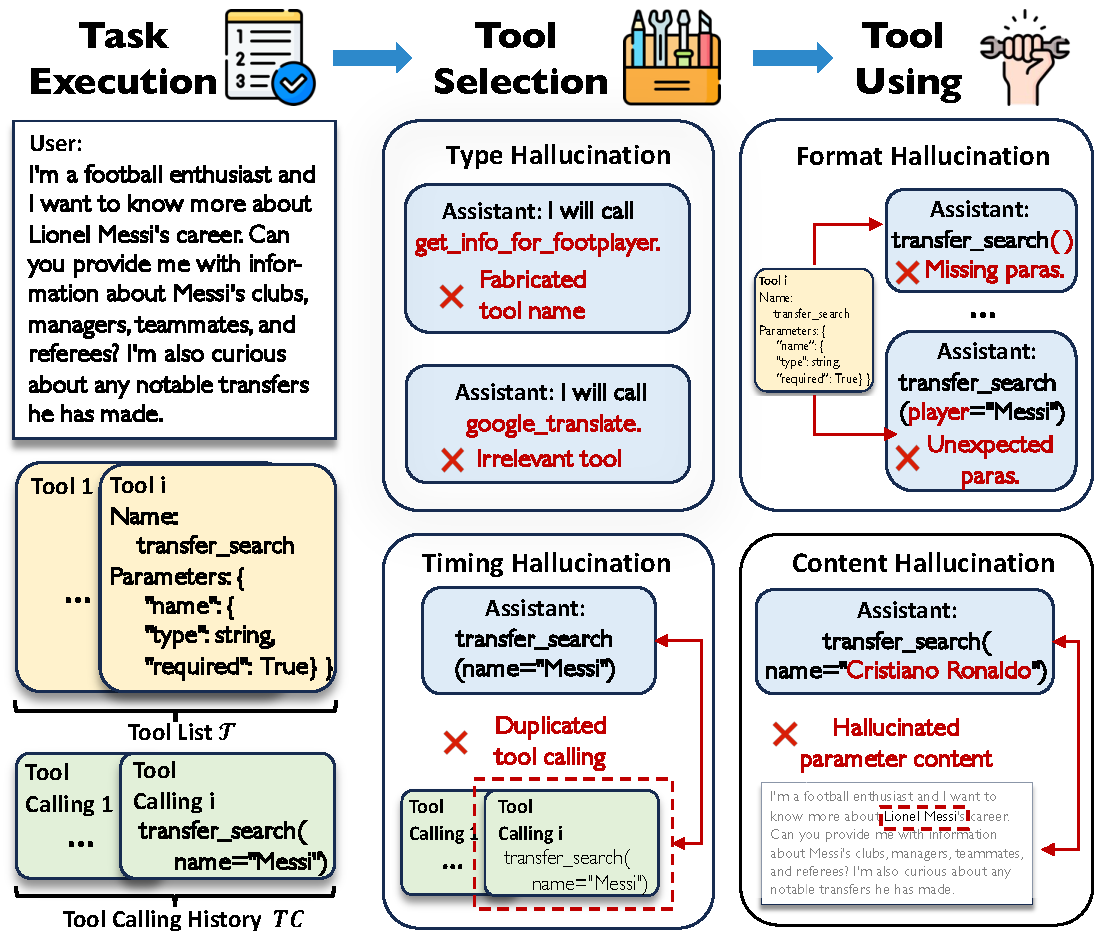
\includegraphics[width=0.48\textwidth]{figs/hallucination_type.pdf}
    \vspace{-6mm}
    \caption{Different types of tool hallucination.}
    % \vspace{-4mm}
    \label{fig:hallucination_type}
\end{figure}

\begin{figure}[t!]
    \centering
    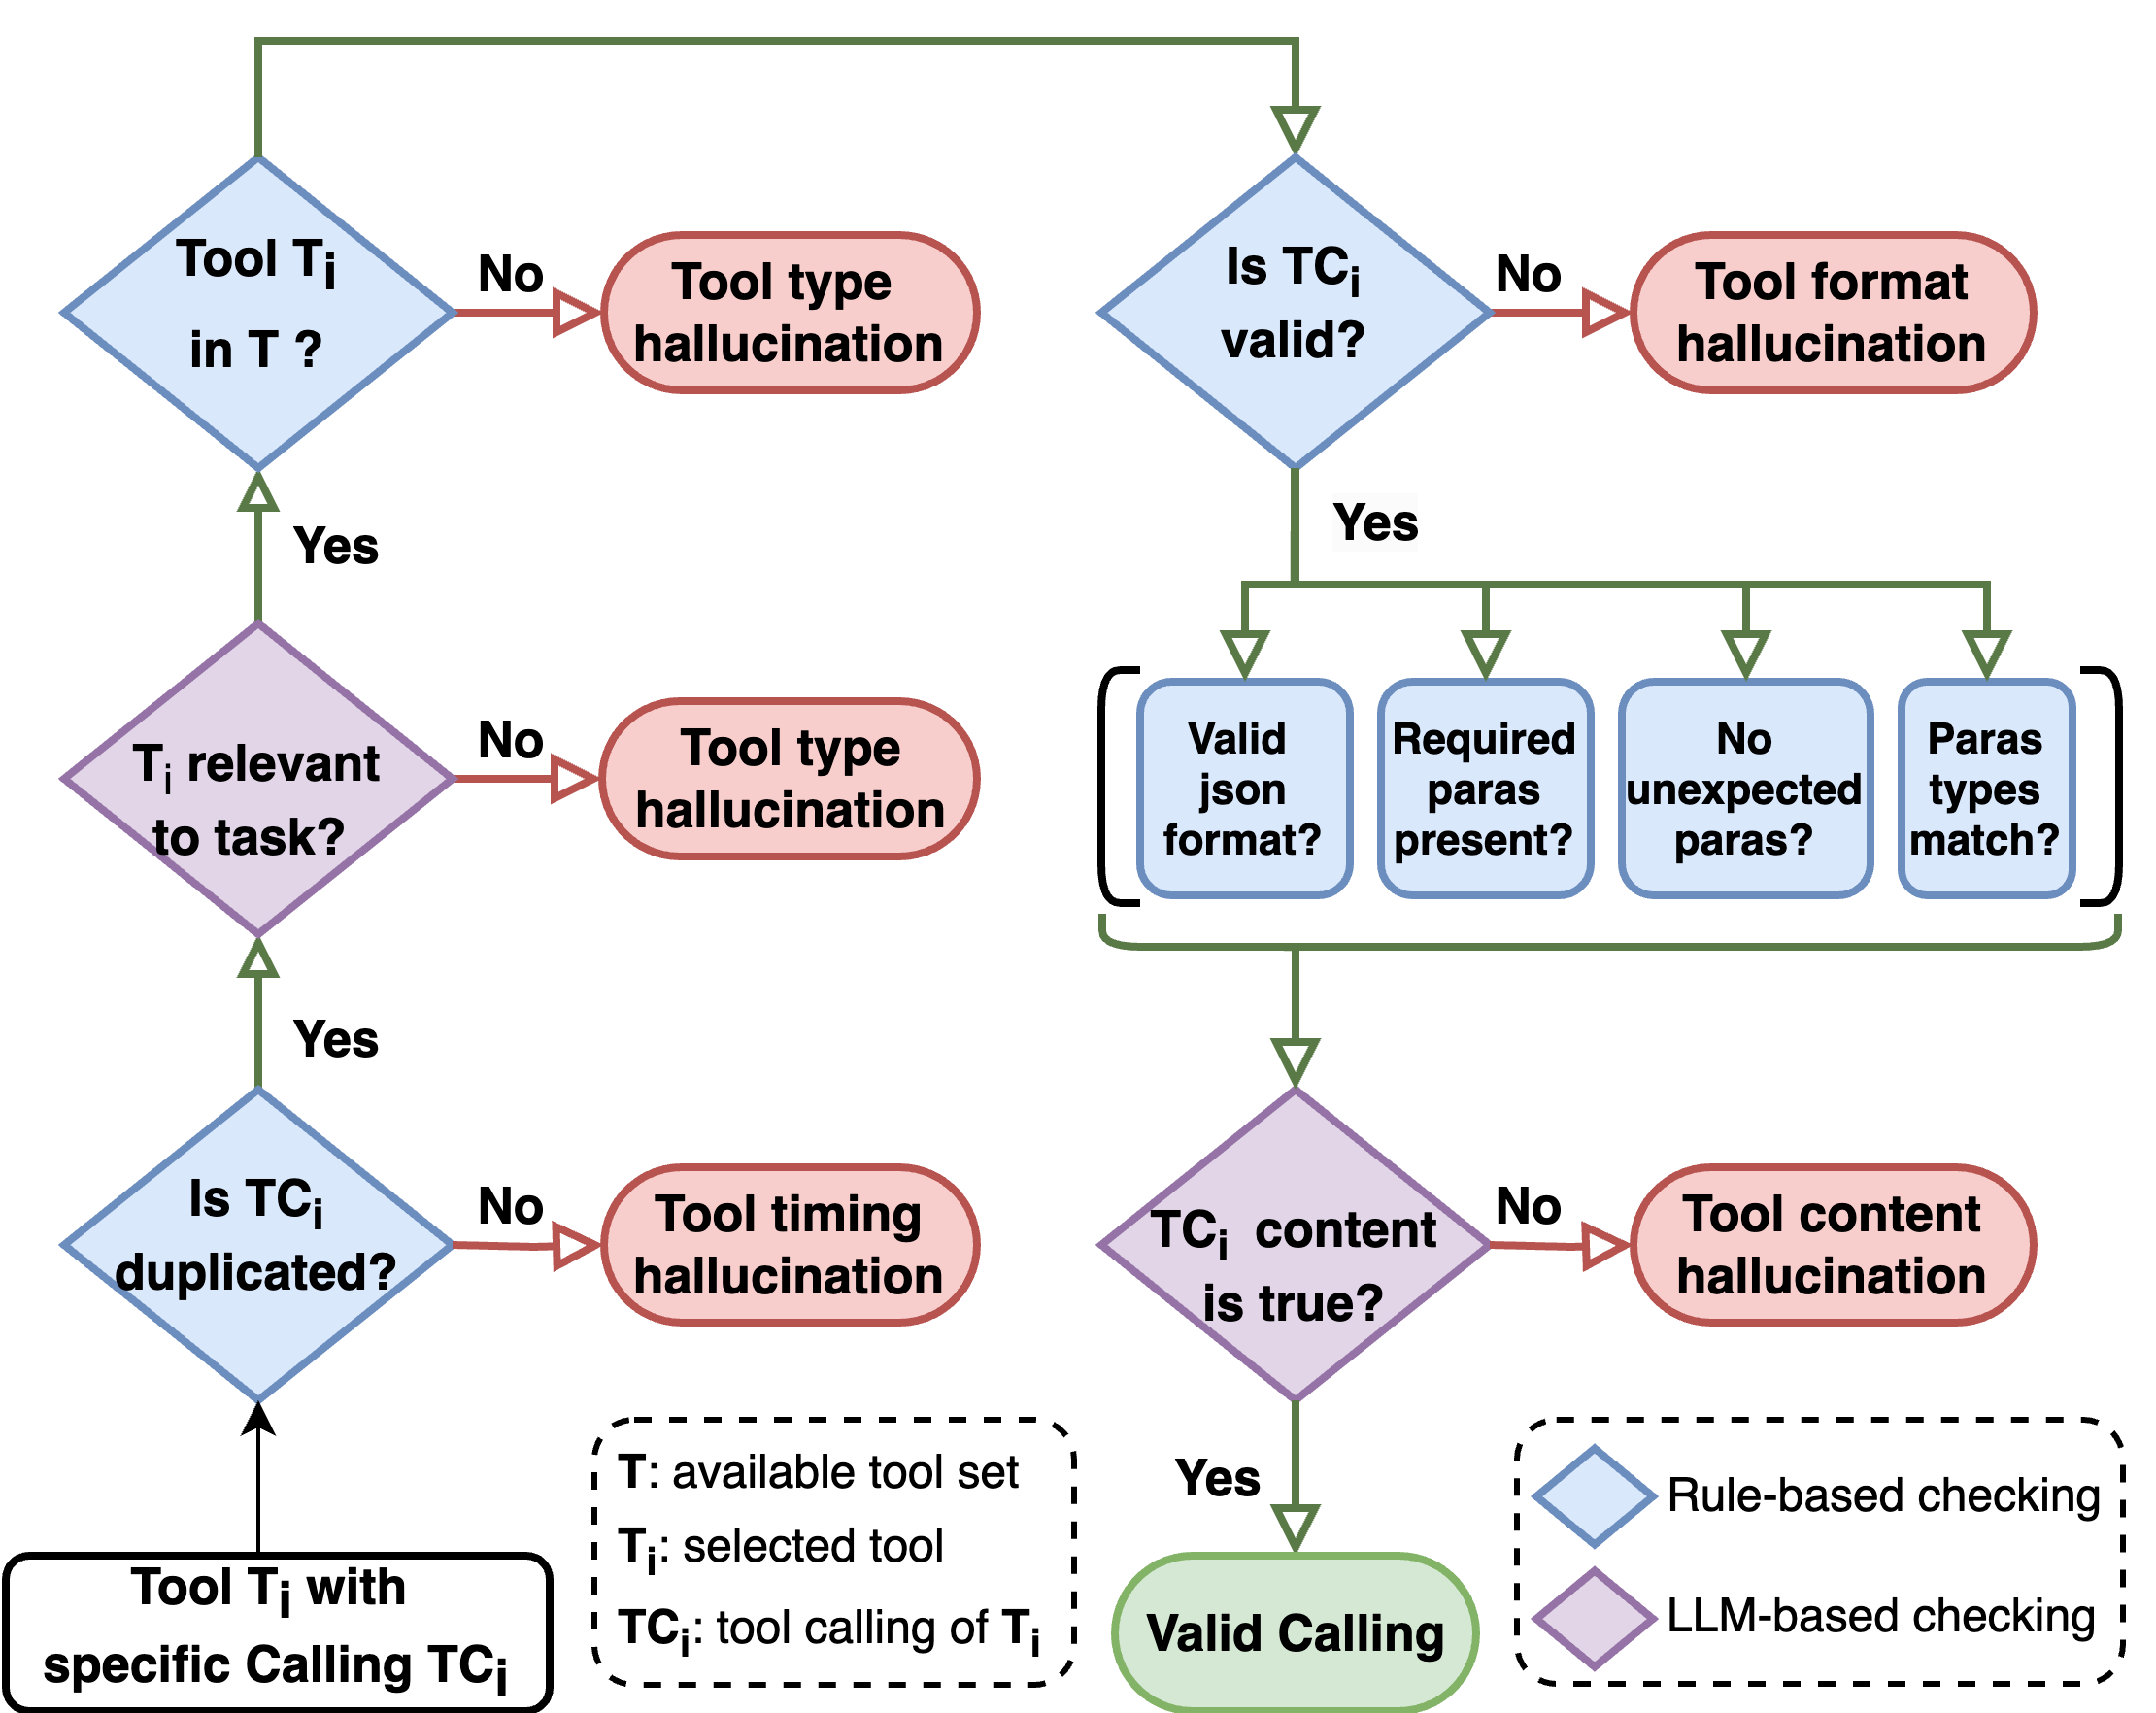
\includegraphics[width=\linewidth]{figs/tool_hallu.png}
    \vspace{-4mm}
    \caption{Evaluation process of tool hallucination.}
    % \vspace{-4mm}
    \label{fig:hallu_eval}
\end{figure}

With the emergence of intelligent agent frameworks like AutoGPT and MetaGPT~\cite{hong2024metagpt}, LLMs now demonstrate enhanced capabilities in real-world interactions through tool use. However, when LLMs interface with external environments via these tools, hallucinations during tool execution can directly affect real-world systems. 

We view tool calling as a decision-making action. When the conditions for making a decision are not met or when the decision fails, it can result in unexpected hallucinations. We categorize the tool hallucination into two major types: 

\textbf{Tool selection hallucination} occurs when the model either selects an inappropriate tool or calls a tool at the wrong time. This category can be further divided into two subtypes: 

\begin{itemize}
    \item \textbf{\textit{Tool type hallucination}} indicates that the model either invokes a tool that is unrelated to the task or fabricates a tool that does not exist in the available tool set.
    \item \textbf{\textit{Tool timing hallucination}} involves errors related to the sequence of tool calling. Specifically, this form of hallucination occurs when the model calls the same tool repeatedly with identical inputs and outputs, indicating that the tool should not have been called again at that point in the task process.
\end{itemize}



\textbf{Tool usage hallucination} pertains to errors in how the model uses a tool after selecting it. This category includes:
\begin{itemize}
    \item \textbf{\textit{Tool format hallucination}} refers to errors in the structure or format of the tool’s usage, such as providing an invalid JSON format, using incorrect parameter names, omitting required parameters, or specifying parameters with values of the wrong data type.
    \item \textbf{\textit{Tool content hallucination}} represents cases where the specific content of the tool’s parameters is fabricated by the model, meaning that the input provided to the tool was not based on the user’s query but was instead invented by the model.
\end{itemize}

We then determine tool hallucinations and their types following the process in Figure~\ref{fig:hallu_eval}. To ensure comprehensive evaluation, we integrate rule-based methods with an LLM evaluator (GPT-4o).   Rule-based methods detect structural errors such as invalid JSON formats and missing parameters. However, assessing tool-task relevance and parameter authenticity requires deeper semantic understanding, which the LLM evaluator provides:  
\begin{itemize}
    \item \textbf{Tool-task relevance assessment.} The evaluator infers a tool’s intended function from its description and parameters, verifying alignment with the user query. It also detects errors in tool invocation timing, such as redundant or premature calls.
    \item \textbf{Parameter authenticity verification.} The evaluator checks whether tool parameters (e.g., user IDs, city names) are derived from the user’s input or fabricated. If a parameter lacks a clear basis in the query, it is classified as a hallucination.  
\end{itemize}

We design structured prompts (Appendix~\ref{sec:prompt_check_relevance}, \ref{sec:prompt_check_content_hallucination}) to guide these evaluations. Human assessment shows that LLM-based evaluation achieves 92.7\% accuracy (Appendix~\ref{sec:human_eval}), closely aligning with expert judgments.  

To quantify hallucinations, we introduce the \textbf{tool hallucination rate}, measuring the proportion of hallucinated tool calls in a given task. For a task with \( N_{\text{total}} \) tool calls and \( N_{\text{hallucination}} \) hallucinated calls, we define:  
\begin{equation*}
H_{\text{sample}} = 
\begin{cases} 
\frac{N_{\text{hallucination}}}{N_{\text{total}}} & \text{if } N_{\text{total}} > 0, \\
0 & \text{otherwise.}
\end{cases}
\end{equation*}  
The task-level hallucination rate is computed as the average sample-level hallucination rate across all task instances, providing an overall measure of tool-use reliability.

% We then determine whether a specific tool calling is hallucinated and identify its type through the process outlined in Figure~\ref{fig:hallu_eval}. It's important to note that we rely not only on rule-based detection like format checking but also leverage LLMs (specifically, GPT-4o) as an evaluator to assess certain aspects of hallucinated tool calls. The LLM plays a crucial role in evaluating the relevance between the tool and the task, as well as determining whether the tool calling parameters are derived from the user's input or fabricated by the model. The evaluation prompts are shown in the Appendix~\ref{sec:prompt_check_relevance},\ref{sec:prompt_check_content_hallucination}.

% Through rigorous human evaluation, we find that the LLM-based automatic evaluation achieves an overall accuracy of 92.7\% (details in Appendix~\ref{sec:human_eval}). This indicates that the LLM evaluator can closely align with human judgment, particularly in determining the relevance of the tool to the task and verifying the origin of tool parameters.



% Consequently, we introduce the \textbf{tool hallucination rate}, a metric designed to capture the proportion of hallucinated tool callings over a set of tasks. This metric first calculates hallucination rates at the sample level—for individual task executions—then averages these rates across all samples to obtain a more comprehensive measure of overall tool hallucination behavior. For a given task, let \( N_{\text{total}} \) represent the total number of tool callings, and \( N_{\text{hallucination}} \) denote the number of hallucinated tool callings. The sample-level tool hallucination rate is defined as:

% \begin{equation*}
% H_{\text{sample}} = 
% \begin{cases} 
% \frac{N_{\text{hallucination}}}{N_{\text{total}}} & \text{if } N_{\text{total}} > 0, \\
% 0 & \text{if no tools were invoked.}
% \end{cases}
% \end{equation*}
% \begin{equation} H_{\text{overall}} = \frac{1}{N_{\text{samples}}} \sum_{i=1}^{N_{\text{samples}}} H_{\text{sample}, i} \end{equation}


% where \( N_{\text{samples}} \) is the total number of tasks in the evaluation set, 


\subsection{Reliability Evaluation}

% While tool hallucinations introduce erroneous executions, their impact extends beyond isolated failures. They contribute to increased decision-making costs, inefficient resource usage, and degraded task reliability. Therefore, evaluating LLM tool use requires a holistic perspective that accounts for both task success and tool efficiency. To capture this balance, we introduce two key metrics:
% 1) Reliable Pass Rate and 2) Benefit-Cost Utility. Together, these metrics provide a comprehensive view of LLM reliability in tool use, moving beyond simple task success rates to evaluate models in real-world, resource-constrained scenarios.


% \subsubsection{Reliable Pass Rate}

% \textit{Reliable Pass Rate} is the proportion of tasks that were successfully passed without hallucinated answers (we refer the readers to ToolBench paper for detailed pass rate evaluation; we use LLM to check if the answer is hallucinated, the prompt is shown in Appendix~\ref{sec:prompt_check_hallucinated_answer}).

In this section, we assess the reliability of tool use in LLMs by introducing two key metrics: \textbf{Reliable Pass Rate (RePR)} and \textbf{Benefit-Cost Utility}. Both metrics offer distinct insights into the model's ability to perform tasks efficiently and accurately while managing tool-related challenges such as hallucinations. The Reliable Pass Rate emphasizes the accuracy of task completion, focusing on the reduction of hallucinations, while the Utility metric incorporates both the success of the task and the associated costs, penalizing excessive tool usage and hallucinations.

\subsubsection{Reliable Pass Rate}

The Reliable Pass Rate (RePR) measures the proportion of tasks successfully completed without hallucinated responses. RePR subtracts the hallucinated outcomes from the standard pass rate, offering a clearer view of a model’s reliability in executing tasks without introducing errors. The formula for calculating RePR is:
$$
\text{RePR} = \text{Pass Rate} - \text{Task Hallucination Rate}.
$$
Here, Pass Rate refers to the proportion of tasks that are successfully completed (for detailed evaluation methods, please refer to the ToolBench paper~\cite{qin2023toolllm}), and Task Hallucination Rate quantifies the proportion of tasks affected by tool hallucinations. Importantly, tasks with an original pass rate of 0 are not considered as having result hallucinations to avoid repeated punishment.  Once tool hallucinations are identified, task hallucination is further assessed by using an LLM to verify whether the known hallucinated tool calls correlate with the final task result (for the prompt, refer to Appendix~\ref{sec:prompt_check_hallucinated_answer}). We also present a comparison between the original pass rate and our RePR metric in Figure~\ref{fig:repr}. We observe that, across different datasets, there are certain result hallucinations that are not directly identifiable by various evaluation models. As a result, our RePR metric is significantly lower than the pass rate.

\begin{figure}[htbp]
    \centering
    % 第一个子图
    \begin{subfigure}[b]{0.23\textwidth}
        \centering
        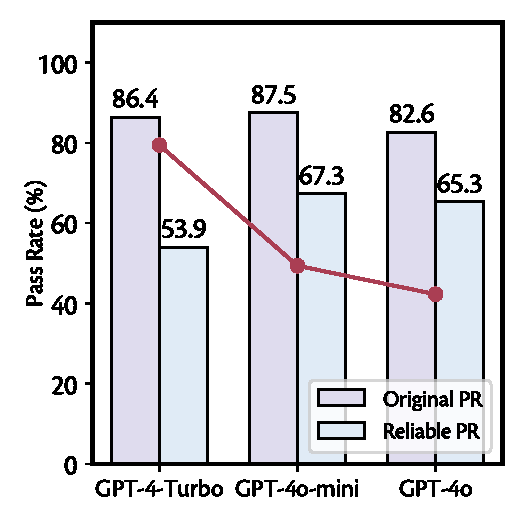
\includegraphics[width=\textwidth,trim=10 10 10 10,clip]{figs/pass_rate_models.pdf}
        % \caption{metric comparison over evaluators}
    \end{subfigure}
        \begin{subfigure}[b]{0.23\textwidth}
        \centering
        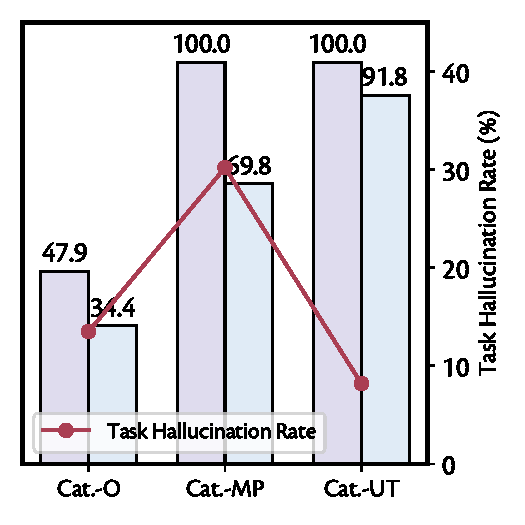
\includegraphics[width=\textwidth,trim=10 10 10 10,clip]{figs/pass_rate_items.pdf}
        % \caption{metric comparison over subsets}
    \end{subfigure}
    \vspace{-0.3cm}
    \caption{Metric comparison between reliable and original pass rate. O, MP, and UT represent the original, missing parameter, and unmatched tools subsets, respectively.}
    \label{fig:repr}
\end{figure}


\subsubsection{Benefit-Cost Utility}

The \textbf{Benefit-Cost Utility} takes a more holistic approach by evaluating both the task outcome and tool usage efficiency. The utility score is designed to reflect the overall quality of task execution, considering not only task success but also the penalties incurred from hallucinations and excessive tool calls. The formula for calculating the utility score is:
$$
\text{Utility} = R_{\text{task}} - P_{\text{tool}} - P_{\text{hallucination}},
$$
where \( R_{\text{task}} \) is the reward based on the task outcome (20 for success, 0 for failure), \( P_{\text{tool}} \) is the penalty for excessive tool usage (calculated as \( \min( \#(total\ tool\ calls) - \#(necessary\ tool\ calls), 10) \)), and \( P_{\text{hallucination}} \) is the penalty for hallucinations in the task (-10 for hallucination). 
Unlike RePR, which focuses solely on the task completion rate after excluding hallucinations, the Utility metric incorporates both the quality of the result and the efficiency of tool usage, making it a more comprehensive measure of tool reliability. It explicitly penalizes hallucinations and excessive tool calls, thus balancing the success rate with the cost of tool inefficiency and errors.

% In summary, while \textbf{RePR} primarily focuses on evaluating the model's ability to complete tasks correctly after excluding hallucinations, the \textbf{Utility} metric provides a broader measure that penalizes both hallucinations and inefficient tool use, offering a deeper insight into the overall reliability and cost-effectiveness of the model's tool interactions.








% \subsubsection{Benefit-Cost Utility}
% The \textbf{benefit-cost utility} serves as a reward-based metric that assigns a score to each task execution based on its outcome and the efficiency of tool usage. The utility captures the quality of the task result (success, failure, or hallucination) as well as the penalty for excessive tool calling. The scoring system is designed to incentivize both high task completion rates and efficient tool usage.


% The utility score for each task execution is therefore:

% \begin{equation}
% \text{Utility} = R_{\text{task}} - P_{\text{tool}}
% \end{equation}

% where $R_{\text{task}}$ is the reward based on task outcome (20 for success, 0 for failure, -10 for hallucination); $P_{\text{tool}}$ is the penalty for excessive tool callings, calculated as $\min( \#(total\ tool \ calls) - \#(necessary\ tool\ calls), 10)$.


\subsection{Construction of RelyToolBench}

To better evaluate tool hallucination and task reliability, we introduce RelyToolBench, which builds upon StableToolBench~\cite{guo2024stabletoolbench}. RelyToolBench extends the original test set by synthesizing two additional categories of subsets designed to simulate challenging conditions for the model. Both of the two categories are critical for evaluating the tool reliability of LLMs in real-world applications.  The dataset statistics are provided in the Table~\ref{tab:data_statistics}. Specifically, we generate two additional subsets:

\begin{itemize}
\item \textbf{Missing Parameter Subset}: This modification obscures certain parameters related to tool callings within the task. Specifically, this data is generated using LLMs to hide parameters within the tasks. This aims to simulate scenarios where crucial tool-related information is hidden, allowing us to evaluate the model’s ability to function effectively under incomplete information. The prompts can be found in the Appendix~\ref{sec:prompt_data_generation}.
\item \textbf{Unmatched Tools Subset}: We replace the tools specified in the task with irrelevant or mismatched tools. This modification tests the model’s ability to handle hallucinations arising from errors in tool selection, where the model may incorrectly identify or call the wrong tool for a given task.
\end{itemize}

% \begin{table}[ht]
% \centering
% \caption{\textbf{Data Statistics for ReleToolBench.} Ori: Original, MP: Missing Parameter, UT: Unmatched Tools.}
% \begin{tabular}{lcccc}
% \toprule
% \multirow{2.5}{*}{\textbf{Subset}} & \multirow{2.5}{*}{\textbf{Solvability}} & \multicolumn{3}{c}{\textbf{Count}} \\
% \cmidrule(lr){3-5}
%  & & \textbf{Ori} & \textbf{MP} & \textbf{UT} \\
% \midrule
% \multirow{2}{*}{I1 Instruction} 
%  & Solvable & 163 & -- & -- \\
%  & Unsolvable & -- & 99 & 163 \\
% \midrule
% \multirow{2}{*}{I2 Category} 
%  & Solvable & 124 & -- & -- \\
%  & Unsolvable & -- & 103 & 124 \\
% \midrule
% \multirow{2}{*}{I3 Instruction} 
%  & Solvable & 61 & -- & -- \\
%  & Unsolvable & -- & 60 & 61 \\
% \bottomrule
% \end{tabular}
% \label{tab:data_statistics}
% \end{table}



\begin{table}[ht]
% \begin{adjustbox}{width=\textwidth}
\centering
% \footnotesize
\caption{\textbf{Data Statistics for RelyToolBench.}}
\resizebox{\columnwidth}{!}{
\setlength\tabcolsep{3pt}
\renewcommand{\arraystretch}{0.8}
\begin{tabular}{cccccc}
\toprule

\multirow{2.5}{*}{\textbf{Category}} & \multirow{2.5}{*}{\textbf{Solvable}} & \multicolumn{3}{c}{\textbf{Subset}} & \multirow{2.5}{*}{\textbf{Total}}\\
\cmidrule(lr){3-5}
 % &  & \makecell{I1 \\Instruction} & \makecell{I2 \\Category} & \makecell{I3 \\Instruction}  &\\
 &  & I1-Inst. & I2-Cat. & I3-Inst.  &\\
\midrule
Original & \Checkmark & 163 & 124 & 61 & 348 \\
Miss Parameter & \XSolidBrush & 99 & 103 & 60 & 262 \\
Unmatched Tools & \XSolidBrush & 163 & 124 & 61 & 348 \\
\midrule
\quad Total & - & 425 & 351 & 182 & 958 \\
\bottomrule
\end{tabular}}
\label{tab:data_statistics}
% \end{adjustbox}
\end{table}




\section{Reliability Alignment}

In this section, we introduce the alignment framework for tool reliability, Relign. As illustrated in Figure 1, Relign consists of three components: the tool-level alignment objectives (\ref{3.1}), the process for synthesizing tool preference data(\ref{3.2}), and the overall training pipeline (\ref{3.2}). We identify the primary cause of tool hallucinations as the model's lack of proper modeling of the decision conditions when making tool-related decisions. Specifically, if an LLM calls a tool under conditions where the decision criteria are not met—such as when the tool's parameters are unknown or when the tool is mismatched with the task—the occurrence of tool hallucinations significantly increases. To address this, we introduce the concept of \textit{indecisive action space}, where alternative actions such as \texttt{ChangeTools} and \texttt{TalkToUser}  when tool invocation conditions are unmet. Furthermore, we enhance the model's awareness of boundary conditions in tool calling by training it with synthesized alignment data.

\begin{figure*}[t!]
    \centering
    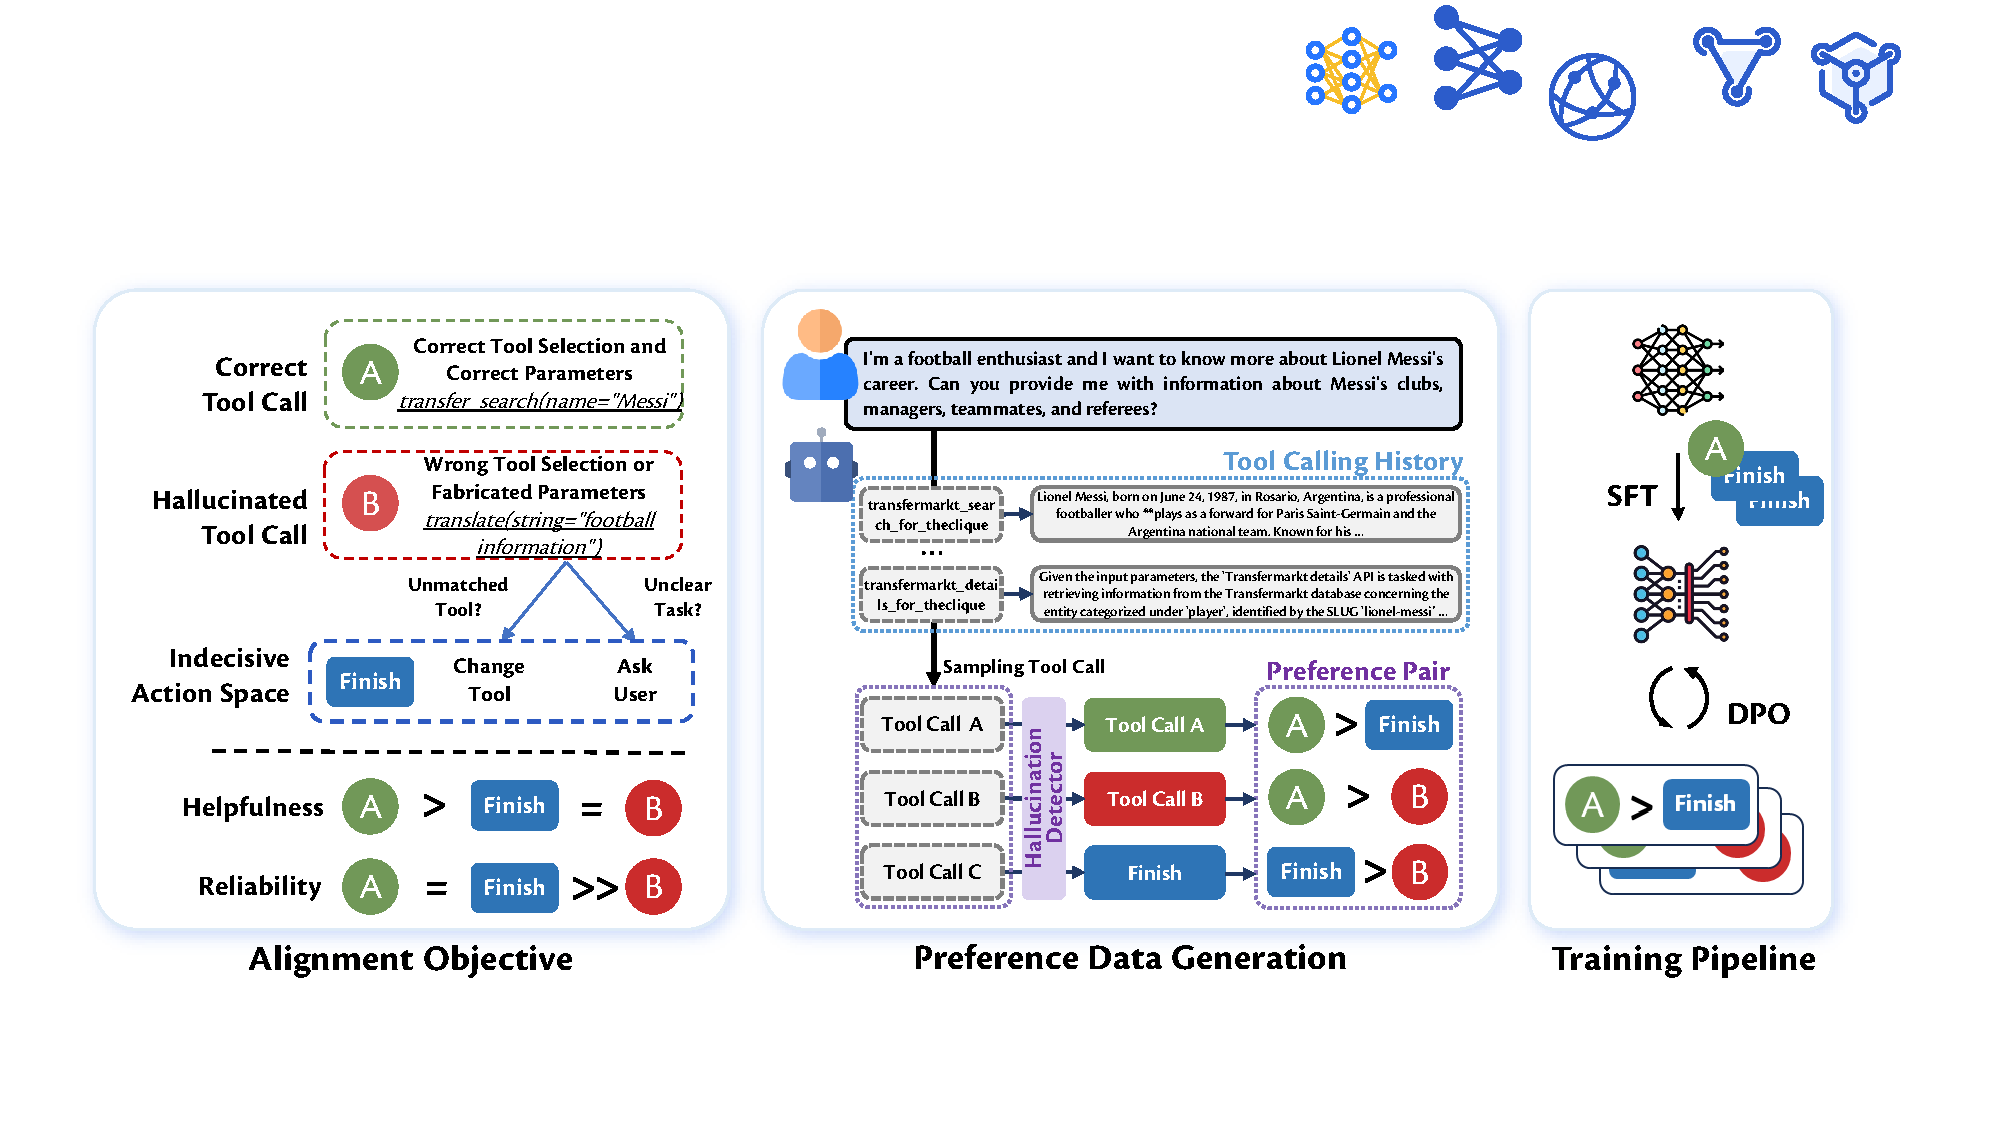
\includegraphics[width=\linewidth,trim=40 70 70 120,clip]{figs/system.pdf}
    \vspace{-6mm}
    \caption{\textbf{The system illustration of Relign.}} 
    \vspace{-4mm}
    \label{fig:system}
\end{figure*}

\subsection{Alignment Goal}
\label{3.1}
% \paragraph{Task-Level Preference Hierarchy}
% At the task completion level, we establish a strict preference ordering based on outcome quality:
% \begin{itemize}
%     \item \textbf{Successful trajectories} ($T_{\text{success}}$) that achieve accurate task completion through valid tool calls are maximally preferred
%     \item \textbf{Aborted trajectories} ($T_{\text{abort}}$) where the model actively terminates execution via indecisive actions (e.g., "Insufficient information to proceed") are intermediately preferred
%     \item \textbf{Hallucinated trajectories} ($T_{\text{hallucination}}$) containing invalid tool calls are strictly penalized
% \end{itemize}

% Formally, this hierarchy satisfies:
% \begin{equation}
%     T_{\text{success}} > T_{\text{abort}} > T_{\text{hallucination}}
% \end{equation}


% 
The alignment goal for reliable tool calling in LLMs focuses on ensuring accurate and effective interactions with external tools throughout the task completion process. From a task perspective, the primary objective is to maximize successful tool calling while minimizing hallucinations. This can be formalized as a preference hierarchy: formally, let $T$ represent a tool calling trajectory, and $H(T)$ the hallucination rate within that trajectory. For a given task, we define the alignment preference as:
$$
T_{\text{success}} > T_{\text{failure}} > T_{\text{hallucination}},
$$
where $T_{\text{success}}$ represents a successful trajectory, $T_{\text{failure}}$ represents a trajectory resulting in task failure or abandonment, and $T_{\text{hallucination}}$ represents a trajectory that generates a hallucinated result.

In our experiments, we observe that when a model exhibits a high rate of tool hallucinations, it tends to favor producing hallucinated outputs rather than acknowledging failure. This behavior poses a significant risk, as hallucinated results may mislead users into believing the task was successfully completed, thus undermining trust in the system.


Therefore, building upon the task-level alignment preference, we define the alignment preference at step level for tool interaction tasks. Specifically, a non-hallucinated tool call is preferred over indecisive actions and hallucinated tool calls. This preference hierarchy can be formalized as:
$$
A_{\text{correct}} > A_{\text{indecisive}} > A_{\text{hallcuinated}},
$$
where $A_{\text{correct}}$, $A_{\text{indecisive}}$, $A_{\text{hallcuinated}}$ represent correct tool calling actions, indecisive actions and hallucinated tool calling actions, respectively. We also find that for many tasks, the number of required tool callings is typically fixed. Models that invoke tools excessively tend to introduce more hallucinations. Thus, minimizing tool hallucination not only improves task reliability but also reduces the overall number of tool callings, leading to more efficient tool usage. 



\subsection{Alignment Methods}
\label{3.2}
The overall data synthesis and alignment training process is illustrated in the middle and right parts of Figure 4. First, we construct reliable supervision data for Supervised Fine-Tuning (SFT) to train the model on the appropriate use of indecisive actions. After the initial SFT training, we sample and synthesize reliable preference data based on the model, which is then used to further train the model through the Direct Preference Optimization (DPO) approach. This two-step process ensures that the model not only learns to handle indecisive actions effectively but also aligns with the desired task-level preferences in the long run.

\subsubsection{Reliable SFT}

% The first step in our approach is Supervised Fine-Tuning (SFT), where we sample tool calling traces for specific tasks. If any of these traces lead to successful task completion, we select those with the fewest hallucinations as the labels for fine-tuning. If all sampled traces fail, we consider that the task might be infeasible for the model and design strategies for rejection based on the hallucination types. Specifically:

% \begin{itemize}
% \item \textbf{Tool Type Hallucinations:} When these types of hallucinations occur, indicating that the available tools are insufficient for the task, the model is trained to trigger a “ChangeTools” function, requesting alternative tools.
% \item \textbf{Tool Content Hallucinations:} If hallucinations are due to incorrect tool content, the model learns to invoke a “TalkToUser” function, signaling task completion through communication.
% \end{itemize}

We observe that among the four types of hallucinations, tool type and content hallucinations occur more frequently. Therefore, the main objective of our Supervised Fine-Tuning (SFT) is to train the model to address these hallucinations by learning to invoke "ChangeTools" for tool type hallucinations and "TalkToUser" for tool content hallucinations. Similar to the data synthesis in RelyToolBench, we select specific samples from ToolBench's training data, modifying them by replacing tool sets or removing tool parameters to simulate these hallucinations. The model is then trained to output the appropriate actions based on these modifications. To ensure the generalizability of the experiment and results, the training data we selected involves only a single tool.

\subsubsection{Reliable DPO}

After obtaining a model capable of outputting indecisive actions through SFT, we further optimize it using Direct Preference Optimization (DPO). Direct Preference Optimization (DPO) focuses on constructing preference data to fine-tune the model’s behavior. The goal of DPO is to guide the model in selecting optimal tool calling traces based on task success and hallucination types. Specifically, for each tool calling trajectory, at any given step, we sample multiple responses and use a hallucination evaluator to categorize these responses into three types: hallucinated tool calling action $A_{hallucinated}$, non-hallucinated tool calling action $A_{coreect}$, and indecisive actions $A_{indecisive}$. Based on these classifications, we generate three types of preference pairs: $(A_{correct}>A_{indecisive})$, $(A_{indecisive}>A_{hallucinated})$, $(A_{correct}>A_{hallucinated})$. For each type of preference pair, we randomly select one from the sampled responses to construct the DPO training data.
% We define preference data across three main scenarios, which dictate how the model ranks different responses:

% \begin{itemize}
% \item \textbf{Successful vs. Unsuccessful Traces:} If there are successful traces for a task, traces with fewer hallucinations are preferred over those with more hallucinations. Additionally, successful traces are always preferred over traces where the model invokes rejection mechanisms such as tool changes or task abandonment.
% \item \textbf{Tool Type Hallucinations:} When the primary hallucination type is tool relevance (i.e., the model incorrectly selects irrelevant tools), traces where the model invokes a “ChangeTools” function are preferred over traces where it persists with hallucinated tool calls.
% \item \textbf{Tool Content Hallucinations:} If the hallucinations are due to incorrect tool content (i.e., the model generates incorrect output based on the tool’s response), traces where the model communicates task difficulties via the “TalkToUser” function are preferred over those that continue using incorrect tool data.
% \end{itemize}

% The ranking preferences can be summarized as:
% $$
% T_{s, l} \succ T_{s, h} \succ T_{f,c} = T_{f, t} \succ T_{f, h},
% $$
% where $T_{s, l}$ and $T_{s, h}$ represent the successful trajectory with relatively low and high tool hallucinations, respectively; $T_{f,c}$ and $T_{f,t}$ represent unsuccessful trajectories where rejection mechanisms with “ChangeTools” and “TalkToUser” function were employed; these are preferred over $T_{f,h}$ with high tool hallucinations or lead to hallucinated outcomes.

The DPO framework ensures that the model learns to rank trajectories according to these preferences. By optimizing over such data, the model becomes capable of choosing the most reliable tool calling sequence or recognizing when to abandon a task or seek further clarification from the user.

% \subsubsection{Joint Training of Reliable SFT and DPO}

% To ensure training stability and maximize model performance, we adopt two joint training strategies that integrate Supervised Fine-Tuning (SFT) and Direct Preference Optimization (DPO). The first approach involves a unified loss function where the losses from SFT and DPO are optimized simultaneously:

% $$
% L_{\text{total}} = \alpha L_{\text{SFT}} + \beta L_{\text{DPO}}.
% $$
 
% This simultaneous optimization stabilizes DPO while leveraging the supervised signals from SFT.

% The second approach involves a sequential process: we first train an SFT model, then sample data from it to generate DPO-specific training data. This allows DPO to build upon the strong foundation of the SFT model, further enhancing performance through preference-based fine-tuning. Both strategies aim to maximize the model’s ability to handle complex tasks, minimize hallucinations, and invoke appropriate rejection strategies.
\section{Experiments}

\begin{table*}[!ht]
    \centering
    % \setlength\tabcolsep{2.9pt}
 % \renewcommand{\arraystretch}{0.9}
 \caption{Performance comparison across different methods. RePR $\uparrow$: reliable pass rate. Tool Hallu $\downarrow$: tool hallucination rate. Tool Num $\downarrow$: average tool calling number. Utility: Benifit-cost utility$\downarrow$.}
 \begin{adjustbox}{width=0.98\textwidth}
    \begin{tabular}{lcccccccccccccccc}
        \toprule
        \multirow{4}{*}{\textbf{Method}} & \multicolumn{4}{c}{\thead{I1 Instruction \\ Solvable + Unsolvable}} & \multicolumn{4}{c}{\thead{I2 Category \\ Solvable + Unsolvable} }& \multicolumn{4}{c}{\thead{I3 Instruction \\ Solvable + Unsolvable}}& \multicolumn{4}{c}{Overall} \\
        \cmidrule(rl){2-5} \cmidrule(rl){6-9} \cmidrule(rl){10-13} \cmidrule(rl){14-17}
        & RePR$\uparrow$ & \thead{Tool \\ Hallu}$\downarrow$ & \thead{Tool \\ Num}$\downarrow$ & Utility$\uparrow$ & RePR$\uparrow$ & \thead{Tool \\ Hallu}$\downarrow$ & \thead{Tool \\ Num}$\downarrow$ & Utility$\uparrow$ & RePR$\uparrow$ & \thead{Tool \\ Hallu}$\downarrow$ & \thead{Tool \\ Num}$\downarrow$ & Utility$\uparrow$ & RePR$\uparrow$ & \thead{Tool \\ Hallu}$\downarrow$ & \thead{Tool \\ Num}$\downarrow$& Utility$\uparrow$ \\
        \midrule
    \rowcolor{gray!8}\multicolumn{17}{c}{\textit{Closed-source LLMs}}\\
     \midrule
     \texttt{gpt-3.5-turbo}  & 66.9 & 57.0 & 5.6 & 8.0 & 57.6 & 64.4 & 7.3 & 4.9 & 50.7 & 68.9 & 11.0 & 2.6 & 58.4 & 63.4 & 8.0 & 5.2 \\
     \texttt{GPT 4o-mini}  & 77.2 & 11.4 & 1.7 & 13.6 & 74.9 & 19.2 & 2.0 & 12.8 & 67.7 & 23.2 & 3.3 & 10.2 & 73.3 & 17.9 & 2.3 & 12.2 \\
     \texttt{GPT 4o}   & 80.1 & 5.9 & 1.2 & 14.8 & 75.1 & 9.6 & 1.3 & 13.3 & 69.1 & 9.5 & 1.8 & 11.9 & 74.8 & 8.3 & 1.4 & 13.4\\
        \midrule
        \rowcolor{gray!8}\multicolumn{17}{c}{\textit{Toolllama (7B)}~\citep{qin2023toolllm}}\\
        \midrule
        \texttt{Baseline} & 64.2 & 55.1 & 3.3 & 8.8 & 64.4 & 56.4 & 3.7 & 8.4 & 58.9 & 57.9 & 4.1 & 6.9 & 62.5 & 56.5 & 3.7 & 8.0 \\
        \texttt{\ \ \  + RLHF}  & 65.1 & 54.2 & 3.2 & 9.0 & 64.6 & 55.7 & 3.5 & 8.7 & 58.5 & 57.5 & 4.1 & 6.7 & 62.7 & 55.8 & 3.6 & 8.1 \\
         \texttt{\ \ \  + Steptool} &67.2 & 53.7 & 3.3 & 10.2 &
         66.8 & 55.9 & 3.7 & 9.4 &
         56.7 & 59.0 & 4.3 &6.2 & 63.6 & 56.2 & 3.8 & 8.6
         \\
         \hdashline
        \texttt{\ \ \  +  SFT}   & 67.8 & 24.8 & 2.1 & 10.8 & 67.6 & 32.7 & 2.6 & 10.3 & 65.7 & 29.6 & 2.5 & 9.9 & 67.0 & 29.0 & 2.4 & 10.3 \\
        \texttt{\ \ \  +  DPO}  & 66.1 & 41.5 & 1.2 & 11.2 & 66.9 & 35.7 & 1.2 & 11.4 & 63.5 & 46.0 & 1.3 & 10.3 & 65.5 & 41.1 & 1.2 & 11.0   \\
        \texttt{\ \ \  +  SFT\&DPO}  & \textbf{71.4} & 25.8 & 2.1 & 11.8 & \textbf{69.0} & 32.4 & 2.5 & 10.9 & 66.6 & 32.1 & 2.5 & 9.9 & 69.0 & 30.1 & 2.4 & 10.9 \\
        \texttt{\ \ \  + Relign}  & 68.2 & \textbf{17.1} & \textbf{0.9} & \textbf{12.2} & 68.3 & \textbf{21.6} & \textbf{0.9} & \textbf{12.2} & \textbf{71.0} & \textbf{16.3} & \textbf{1.0} & \textbf{13.0} & \textbf{69.1} & 1\textbf{8.3} & \textbf{0.9} & \textbf{12.4}   \\
        \midrule
        \rowcolor{gray!8}\multicolumn{17}{c}{\textit{Llama3.1 (8B)}~\citep{dubey2024llama}}\\
        \midrule
        \texttt{Baseline}     & 68.5 & 51.2 & 2.1 & 10.5 & 66.1 & 51.7 & 2.3 & 9.4 & 61.3 & 49.6 & 2.4 & 8.3 & 65.3 & 50.8 & 2.2 & 9.4 \\
        \texttt{\ \ \  + RLHF}     & 68.5 & 51.7 & 2.4 & 10.2 & 66.5 & 50.8 & 2.6 & 9.4 & 61.0 & 49.1 & 2.7 & 7.9 & 65.3 & 50.5 & 2.6 & 9.2 \\
        \texttt{\ \ \  + Steptool}    & 71.1 & 50.8 & 2.0 & 11.2 & 69.7 & 52.0 & 2.3 & 10.5 & 56.3 & 55.8 & 2.5 & 6.8 & 65.7 & 52.9 & 2.3 & 9.5 \\
        \hdashline
        \texttt{\ \ \  +  SFT}  & 71.6 & 17.3 & 1.4 & 12.1 & 71.3 & 24.2 & 1.7 & 11.8 & 66.0 & 28.6 & 2.1 & 9.7 & 69.6 & 23.4 & 1.7 & 11.2 \\
        \texttt{\ \ \  +  DPO} & 69.6 & 43.3 & 2.0 & 11.8 & 67.2 & 44.9 & 2.2 & 11.1 & 62.2 & 50.2 & 2.7 & 9.0 & 66.3 & 46.1 & 2.3 & 10.6   \\
        \texttt{\ \ \  +  SFT\&DPO}  & 77.2 & 14.0 & 1.4 & 13.5 & 72.5 & \textbf{19.0} & 1.6 & 11.5 & 71.5 & 20.1 & 2.0 & 10.9 & 73.7 & 17.7 & 1.7 & 12.0 \\
        \texttt{\ \ \  +  Relign }     & \textbf{80.5} & \textbf{8.7} & \textbf{1.3} & \textbf{14.5} & \textbf{75.8} & 22.1 & \textbf{1.6} & \textbf{12.5} & \textbf{75.3} & \textbf{13.1} & \textbf{1.8} & \textbf{12.4} & \textbf{77.2} & \textbf{14.6} & \textbf{1.5} & \textbf{13.2} \\
        \midrule
        \rowcolor{gray!8}\multicolumn{17}{c}{\textit{Qwen2.5 (7B)}~\citep{yang2024qwen2}}\\
        \midrule
        \texttt{Baseline}    & 71.5 & 46.1 & 2.2 & 10.9 & 66.2 & 49.6 & 2.4 & 9.4 & 57.7 & 51.9 & 2.7 & 6.8 & 65.1 & 49.2 & 2.4 & 9.1 \\
        \texttt{\ \ \  + RLHF}  & 67.8 & 48.7 & 2.3 & 10.7 & 65.4 & 47.3 & 2.4 & 9.8 & 62.8 & 49.4 & 2.6 & 9.6 & 65.3 & 48.5 & 2.5 & 10.0  \\
        \texttt{\ \ \  + Steptool}   & 69.5 & 46.8 & 2.4 & 10.2 & 69.6 & 46.6 & 2.5 & 10.2 & 62.7 & 46.0 & 2.8 & 8.0 & 67.3 & 46.5 & 2.6 & 9.5 \\
         \hdashline
        \texttt{\ \ \  +  SFT} & 69.9 & 18.7 & 1.5 & 11.6 & 69.9 & 25.2 & 1.7 & 11.4 & 62.7 & 33.1 & 2.0 & 8.8 & 67.5 & 25.7 & 1.7 & 10.6  \\
        \texttt{\ \ \  +  DPO}  & 69.9 & 45.0 & 2.3 & 10.6 & 68.7 & 45.5 & 2.4 & 10.0 & 65.2 & 45.9 & 2.9 & 8.7 & 67.9 & 45.4 & 2.5 & 9.8   \\
        \texttt{\ \ \  +  SFT\&DPO}   & 69.8 & 20.6 & 1.5 & 11.4 & 69.7 & 25.8 & 1.7 & \textbf{11.3} & 58.8 & 27.6 & 2.0 & 8.0 & 66.1 & 24.7 & 1.7 & 10.2 \\
        \texttt{\ \ \  + Relign} & \textbf{77.0} & \textbf{12.0} & \textbf{1.3} & \textbf{13.3} & \textbf{69.0} & \textbf{22.6} & \textbf{1.7} & 10.6 & \textbf{72.9} & \textbf{18.3} & \textbf{2.0} & \textbf{11.6} & \textbf{73.0} & \textbf{17.6} & \textbf{1.7} & \textbf{11.9}  \\
        \bottomrule
    \end{tabular}%
    \end{adjustbox}
\label{table:main_res}
\end{table*}
% \input{tables/benifit_cost_ratio.tex}


\subsection{Experimental Setup}

\paragraph{Datasets.} In our experiments, we primarily utilized three datasets:  \textbf{ToolBench}, \textbf{StableToolBench} and \textbf{RelyToolBench}. ToolBench~\cite{qin2023toolllm} was constructed by scraping various APIs from RapidAPI and generating corresponding tasks and executions, comprising a total of 120,000 data samples. StableToolBench~\cite{guo2024stabletoolbench} is a selected subset of solvable samples from ToolBench, and it also proposed a stable environment for evaluation.  We randomly select 10,000 samples from Toolbench for constructing reliability alignment data. We further construct RelyToolBench based on StableToolBench for evalution.

% ToolBench is utilized for training purposes, from which we extracted 10,000 samples to construct our Reliable Alignment training dataset. In addition to these samples, we also randomly sampled a portion of the data to introduce additional tool replacements and construct missing parameters, similar to the evaluation of StableToolBench.

\paragraph{Baselines.} (1) \textbf{RLHF \& StepTool.}  The two baselines are proposed in Steptool~\cite{yu2024steptool}, which augments tool learning by introducing step-level rewards. RLHF is a simplified reinforcement learning version of Steptool with only trajectory-level reward. (2) \textbf{SFT \& DPO.} We also implemented a joint training approach that combines SFT and DPO losses on the same base model as baseline. The combination ratio is set to 0.5.


%SFT learns from correct tool-call traces, while DPO ranks trajectories based on hallucination severity. Their combination enhances tool-use stability and reduces invalid calls. %我们实现了基于同一个基座模型，同时使用DPO和SFT的loss进行混合训练

% \paragraph{Relign.}  
% Relign expands the action space, allowing deferrals and corrections to mitigate hallucinations. It integrates preference optimization and structured training to improve reliability and efficiency.


\paragraph{Training and inference details.}
We use \textsc{Llama-3.1-8B-Instruct}, \textsc{Qwen-2.5-7B-Instruct}, and \textsc{Toolllama 7B}~\cite{qin2023toolllm} as our experimental models. Since LLaMA and Qwen models struggle with complex tool-calling tasks, we fine-tune them using 5,000 instances randomly sampled from ToolBench as the baseline. For all the experiments, we set the training batch size to 32, and the max sequence length to 8192. We utilize the \textsc{DeepSpeed-Chat} framework for efficient model training.  In all methods, the learning rate is set to 1e-5 for SFT and 1e-5 for DPO to ensure consistency, with all training conducted over two epochs. We did not perform a grid search but used standard hyperparameters for all experiments to ensure stable fine-tuning and consistent results.

To construct the SFT training data, we randomly split 10,000 samples into three subsets: 4,000 remain unchanged, 3,000 are modified by replacing tool choices, and 3,000 are used to construct missing parameter cases. The model is directly fine-tuned on these curated tool-call traces. For DPO data construction, we start with the same 10,000 tasks and allow multi-round interactions with the environment. In each round, we sample ten tool-use trajectories at a temperature of 0.7 and use \textsc{GPT-4o} as a hallucination evaluator to construct preference pairs. To ensure data diversity, we retain at most one trajectory per step for each preference combination. While the SFT dataset size remains fixed, DPO training steps vary depending on the number of valid preference pairs. Not all interaction rounds yield usable DPO samples, resulting in a total of 10,000 to 20,000 preference pairs in practice. For instance, Relign training yields 17,000, 19,000, and 14,000 pairs for Toolllama, Llama3.1, and Qwen2.5, respectively. We train with a batch size of 32 for two epochs, with the final number of training steps determined by the number of collected DPO pairs.

Additionally, evaluations regarding tool hallucinations and task success were performed using the \textsc{GPT-4o} model, and other evaluation details follow the setup in StableToolBench~\cite{qin2023toolllm}. The prompt for evaluating StableToolBench across all models is provided in Appendix~\ref{sec:evaluating_stabletoolbench}. For computing both benefit-cost utility, the necessary tool calling number is set to 1 for solvable tasks (original subsets) and 0 for unsolvable tasks ( missing parameter and unmatched tools subsets). We conduct all experiments using Nvidia A800 GPUs.


\subsection{Main Results}
\begin{figure*}[t!]
    \centering
    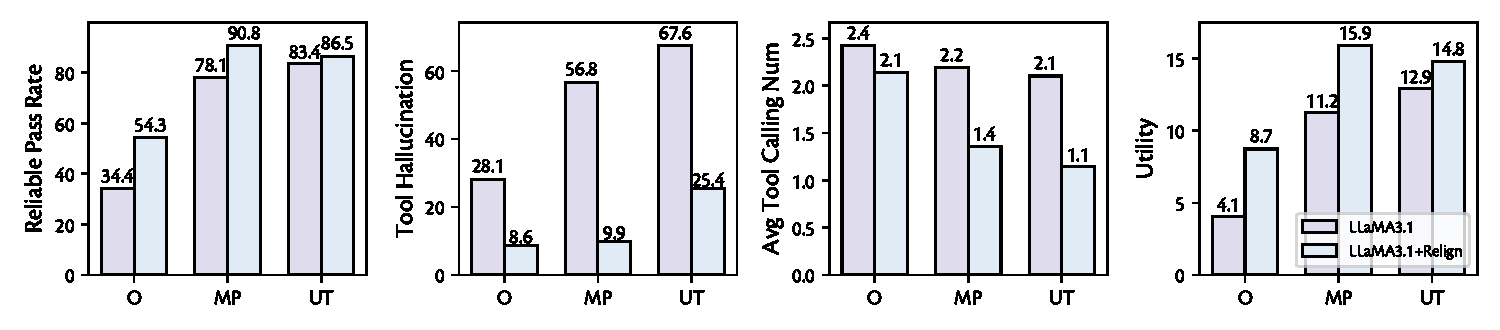
\includegraphics[width=\linewidth]{figs/metrics_grouped.pdf}
    \vspace{-10mm}
    \caption{Comparison of performance metrics between the baseline and Relign across three subsets: Original (O), Missing Parameter (MP), and Unmatched Tools (UT).}
    \label{fig:main_results}
\end{figure*}


\begin{figure}[t!]
    \centering
    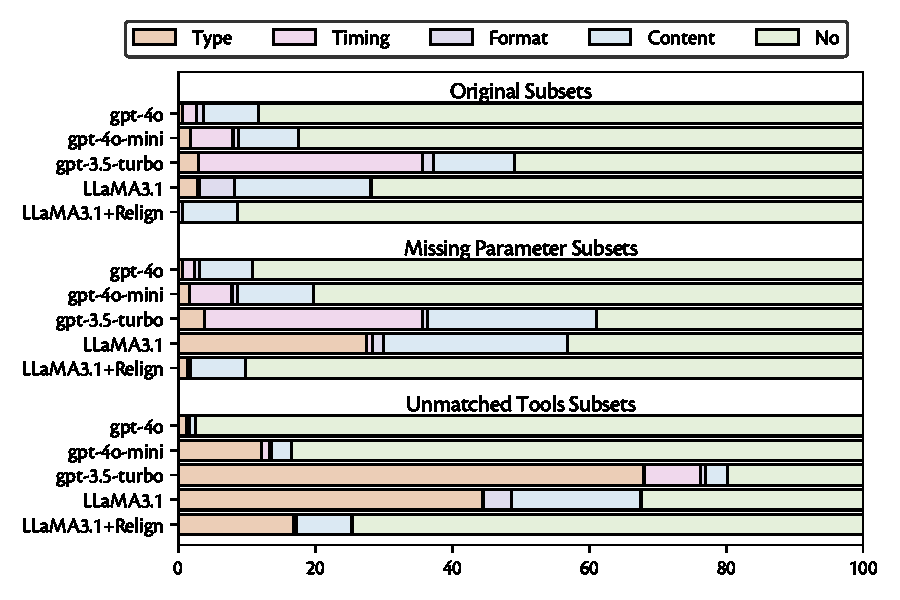
\includegraphics[width=\linewidth,trim=10 10 10 10,clip]{figs/hallu_dist.pdf}
    \vspace{-4mm}
    \caption{\textbf{Distribution of tool hallucination types.} The results highlight the effectiveness of Relign in reducing hallucination across all subsets.}
    \label{fig:hallu_type}
\end{figure}

% \begin{figure}[t!]
%     \centering
% 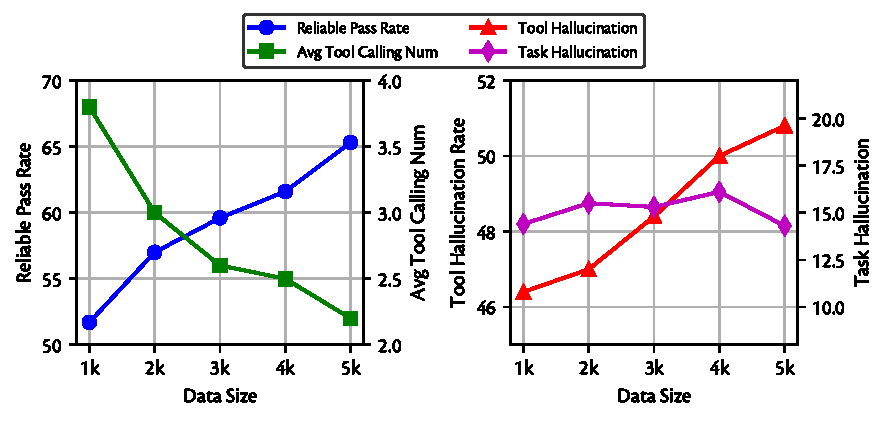
\includegraphics[width=\linewidth,trim=5 5 5 5,clip]{figs/metrics_data_size.pdf}
%     \vspace{-4mm}
%     \caption{\textbf{Comparison of performance metrics between different training data sizes.}}
%     \label{fig:data_size}
% \end{figure}

% \begin{figure}[t!]
%     \centering
% 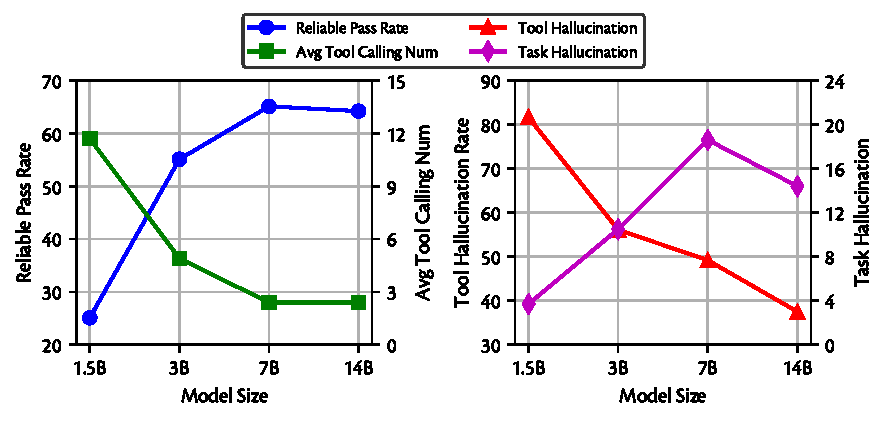
\includegraphics[width=\linewidth,trim=5 5 5 5,clip]{figs/metrics_model_size.pdf}
%     \vspace{-4mm}
%     \caption{\textbf{Comparison of performance metrics between different model sizes.}}
%     \label{fig:model_size}
% \end{figure}

As shown in Table~\ref{table:main_res}, we assessed the performance of our model on three subsets of StableToolbench. Our primary focus was on measuring the tool hallucination rate and the task pass rate. Our results indicate that the implementation of the Reliability Alignment framework, which includes both SFT and DPO, significantly reduces the tool hallucination rate of the baseline model. Moreover, we observed a decrease in the average number of tool callings required for each task. Although previous tool-learning methods, such as StepTool, effectively improve task success rates, they provide no reduction in tool hallucination rates and do not decrease the number of tool calls. In contrast, our approach not only enhances task success rates but also significantly reduces hallucinations. Furthermore, our Relign-trained model based on LLaMA 3.1 outperforms many closed-source models of similar scale, such as GPT-3.5-Turbo and GPT-4o Mini, approaching the performance of GPT-4o.


Figure~\ref{fig:main_results} further demonstrates the effectiveness of our Relign framework in reducing tool hallucination and improving system efficiency across three categories of subsets: Original (O), Missing Parameter (MP), and Unmatched Tools (UT). Relign achieves a remarkable and consistent improvement in all the metrics over all subsets. 
% Our method achieves a remarkable improvement in the Reliable Pass Rate, particularly in the UT subset, where the rate increases from 90.5\% in the baseline to 97.8\%. Similarly, the Tool Hallucination rate experiences a drastic reduction, dropping from 83.0\% to only 4.3\% in the UT subset, highlighting the robustness of our approach in handling mismatched tools. Furthermore, the Average Tool Calling Number decreases significantly across all subsets, with the UT subset seeing a reduction from 4.0 calls in the baseline to just 0.2 calls, showcasing the enhanced ability to reject unmatched tool usage. Finally, our framework maximizes task Utility, with the UT subset showing a substantial increase from 13.8 in the baseline to 19.2, underscoring the practical benefits of our alignment strategies in achieving both reliable and resource-efficient task execution.


% \subsection{Reliability Evaluation}

% Table 2 presents the comprehensive results of the reliability evaluation across different models and methods. In this table, we focus on two key metrics: \textbf{Utility} and \textbf{Ratio}. From the data, it is evident that our proposed approach significantly improves both the utility and ratio compared to the baseline models. Although the combination of SFT and DPO slightly reduces the task pass rate, the substantial reduction in tool hallucinations and unnecessary tool callings leads to a marked increase in both utility and ratio. This improvement indicates better system reliability, as the model becomes more efficient in task completion with fewer errors related to tool usage. The higher utility and ratio values demonstrate that our alignment method not only reduces hallucinations but also enhances the system’s effectiveness in reliably handling complex tasks. 

% \input{tables/hallucination_type.tex}

\subsection{Tool Hallucination Analysis}
Figure~\ref{fig:hallu_type} provides a detailed distribution of different types of tool hallucinations. With Relign framework, all hallucination types show significant reductions, with the greatest improvement observed in the Content Hallucination category, particularly in the Unmatched Tools subset. However, Timing Hallucination demonstrates a relatively smaller improvement, likely due to the inherent difficulty in learning the sequential dependencies required to avoid repetitive or redundant tool calls. This underscores the robustness of our method while identifying areas for further optimization.

% Specifically, within the I1 instruction subset, the predominant hallucinations are tool timing hallucination and tool content hallucination. In the Missing Parameter subset, Tool Content Hallucination is the most common type of error, while in the Unmatched Tools subset, tool type Hallucination dominates. Experimental results demonstrate that our alignment framework enables the model to learn how to accurately assess both the purpose and correct usage of tools, significantly reducing hallucinations in tool selection and usage, and thereby improving the overall reliability of tool callings. Across all subsets, the method demonstrates a consistent reduction in the occurrence of various types of hallucinations. Notably, in the Unmatched Tool subset, our model successfully eliminates hallucinations entirely, bringing the hallucination rate to zero. This significant improvement enhances the reliability of tool usage across the entire subset and reduces hallucination-related errors, ultimately contributing to more accurate and dependable tool interactions.

\subsection{Comparison with Existing Metrics}
Our RePR metric is a refined version of Pass Rate, as we found that some tasks in the original pass rate metric exhibited result hallucinations. Therefore, we believe the pass rate has certain inaccuracies and did not include its results in our paper. As shown in the Table~\ref{table:existing_metrics}, we have supplemented some of the original Pass Rate results. The results indicate that RePR is lower than Pass Rate, and the gap is more pronounced in base models without Relign alignment. This suggests that unaligned models tend to produce more tool hallucinations, which in turn mislead the final results. Moreover, whether using Pass Rate or RePR, our Relign framework consistently improves task success rates.

\begin{table}[!ht]
\centering
\setlength\tabcolsep{3pt}
\resizebox{\columnwidth}{!}{%
\begin{tabular}{lcccccccc}
\toprule
\multirow{2}{*}{\centering Method} & \multicolumn{2}{c}{I1 Instruction} & \multicolumn{2}{c}{I2 Category} & \multicolumn{2}{c}{I3 Instruction} & \multicolumn{2}{c}{Overall} \\
\cmidrule(lr){2-3} \cmidrule(lr){4-5} \cmidrule(lr){6-7} \cmidrule(lr){8-9}
& PR & RePR & PR & RePR & PR & RePR & PR & RePR \\
\midrule
ToolLLaMA         & 76.8 & 64.2 & 77.0 & 64.4 & 72.3 & 58.9 & 75.4 & 62.5 \\
\quad\quad + Relign    & 77.1 & 68.2 & 77.3 & 68.3 & 76.2 & 71.0 & 76.9 & 69.1 \\
\midrule
LLaMA3.1          & 83.0 & 68.5 & 84.8 & 66.1 & 80.1 & 61.3 & 82.6 & 65.3 \\
\quad\quad + Relign    & 87.0 & 80.5 & 89.2 & 75.8 & 86.9 & 75.4 & 87.7 & 77.2 \\
\midrule
Qwen2.5           & 86.3 & 71.5 & 84.3 & 66.2 & 80.6 & 57.7 & 83.7 & 65.1 \\
\quad\quad + Relign    & 87.6 & 77.0 & 87.5 & 69.0 & 85.5 & 72.9 & 86.9 & 73.0 \\
\bottomrule
\end{tabular}%
}
\caption{Comparison of models on original Pass Rate and RePR.}
\label{table:existing_metrics}
\end{table}

\subsection{Out-of-distribution Generalization to APIBench}
As shown in the table below, we also evaluate our method on the out-of-domain test set APIBench. We follow the evaluation setup described in ~\citep{qin2023toolllm} (for more details, please refer to ~\citealp{qin2023toolllm}). Rather than training on APIBench, we treat each API in the prompt as a function call to assess how well our trained model generalizes to OOD datasets. Experimental results with two types of tool retrieval indicate that Relign improves model performance on other tool-use tasks as well, suggesting that reducing tool hallucinations helps models learn better tool-use strategies (AST represents tool-calling accuracy).
\begin{table}[!ht]
\centering
\setlength\tabcolsep{3pt}
\resizebox{\columnwidth}{!}{
\begin{tabular}{lcccccc}
\toprule
\multirow{2}{*}{\centering Method} & \multicolumn{2}{c}{HuggingFace} & \multicolumn{2}{c}{TorchHub} & \multicolumn{2}{c}{Tensorhub} \\
\cmidrule(lr){2-3} \cmidrule(lr){4-5} \cmidrule(lr){6-7}
& Hallu.($\downarrow$) & AST($\uparrow$) & Hallu.($\downarrow$) & AST($\uparrow$) & Hallu.($\downarrow$) & AST($\uparrow$) \\
\midrule
LLaMA3.1 + BM25          & 9.7 & 14.3 & 11.7 & 47.8 & 10.5 & 40.3 \\
\quad + Relign + BM25    & \textbf{6.4} & \textbf{15.7} & \textbf{7.9}  & \textbf{50.1} & \textbf{5.5}  & \textbf{42.5} \\
\midrule
LLaMA3.1 + Oracle        & 9.3 & 87.8 & 10.4 & 86.1 & 7.8  & 89.6 \\
\quad + Relign + Oracle  & \textbf{6.5} & \textbf{89.5} & \textbf{7.7}  & \textbf{88.9} & \textbf{3.2}  & \textbf{91.3} \\
\bottomrule
\end{tabular}
}
\caption{OOD generalization experiments on APIBench.}
\label{table:apibench}
\end{table}


\subsection{Discussion}

\begin{figure}[t!]
    \centering
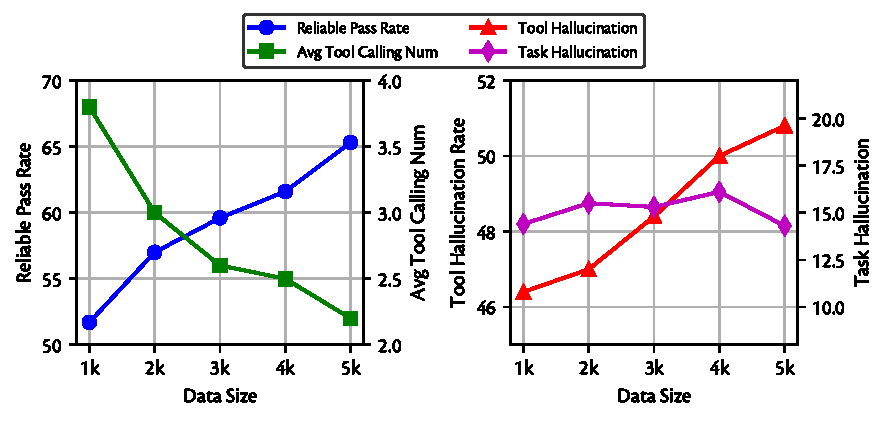
\includegraphics[width=\linewidth,trim=5 5 5 5,clip]{figs/metrics_data_size.pdf}
    \vspace{-4mm}
    \caption{\textbf{Impact of Training Data Size on Performance and Hallucination Metrics.} Experiments are conducted on LLaMA3.1.}
    \vspace{-4mm}
    \label{fig:data_size}
\end{figure}

\paragraph{Does More Data Reduce Hallucination?}
Increasing the amount of training data from 1k to 5k consistently improves model performance, as reflected by the rising Reliable Pass Rate in Figure~\ref{fig:data_size}. However, this increase in data size does not always lead to a reduction in hallucination rates. Both Tool and Task Hallucination rates remain stable or even slightly increase with more data. This could be attributed to overfitting on ToolBench data, which consists of well-structured tool interaction trajectories and lacks samples that handle edge cases (e.g., failure scenarios where a task cannot be completed). Thus, the model learns correct tool calls but struggles with failure scenarios, defaulting to excessive hallucinated tool calls instead of invoking indecisive actions—precisely the issue Relign aims to address.

\begin{figure}[t!]
    \centering
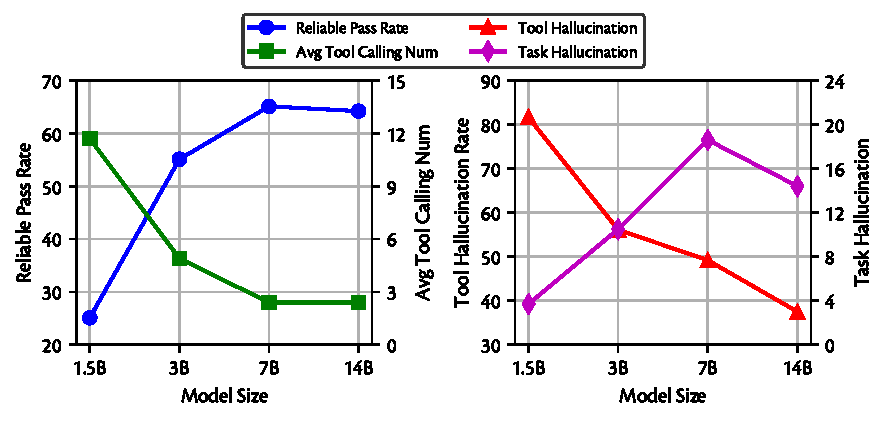
\includegraphics[width=\linewidth,trim=5 5 5 5,clip]{figs/metrics_model_size.pdf}
    \vspace{-4mm}
    \caption{\textbf{Impact of Model Size on Performance and Hallucination Metrics.} Experiments are conducted on Qwen2.5 with 5k data.}
    \vspace{-4mm}
    \label{fig:model_size}
\end{figure}

\paragraph{Does a Larger Model Reduce Hallucination?}
Scaling up model size from 1.5B to 14B, while keeping the training data fixed at 5k, leads to significant improvements in both performance and hallucination reduction, as seen in Figure~\ref{fig:model_size}. Larger models exhibit a better ability to capture complex task dependencies and context, resulting in a noticeable decline in both tool hallucinations and excessive tool calls, leading to more reliable and efficient tool use. Moreover, the Reliable Pass Rate increases with model size, highlighting the enhanced robustness and generalization capabilities of larger models. These results suggest that scaling model parameters is a key strategy for improving the reliability and accuracy of tool usage in complex environments.


\section{Related Work}
\subsection{Tool Learning}
Recent advancements in tool learning have enabled LLMs to effectively integrate external tools, enhancing real-time knowledge retrieval, multimodal functionalities, and domain-specific expertise ~\citep{yang2023chatgpt, gupta2023visual, jin2023genegpt}. Methods range from leveraging in-context learning for tool descriptions and demonstrations~\citep{hsieh2023tool} to explicit training on tool-enriched datasets~\citep{patil2023gorilla, tang2023toolalpaca, qin2023toolllm}. Evaluation of tool-augmented LLMs primarily focuses on metrics like tool call accuracy and task success~\citep{zhuang2023toolqa, guo2024stabletoolbench}, often emphasizing execution over other factors. However, limited research has addressed the critical issue of tool hallucinations~\citep{patil2023gorilla, chen2023teval} and tool efficiency~\citep{xu2025alignment}, which can undermine the reliability and trustworthiness of tool usage in real-world applications.

\subsection{Mitigating Halucinations}
LLMs are prone to generating hallucinations — errors where content conflicts with user inputs, prior generated information, or world knowledge~\citep{guerreiro2023hallucinations, mundler2023self, min2023factscore}. Strategies to mitigate these issues include improving pre-training data quality~\citep{penedo2023refinedweb, touvron2023llama}, fine-tuning with curated datasets~\citep{chen2023alpagasus, zhou2023lima}, using external knowledge sources to ground responses~\citep{gao2023retrieval,jain2024mitigating}, designing better decoding strategies~\citep{shi2023trusting} and estimating uncertainty~\citep{azaria2023internal, xiong2023can, zhao2023verify,varshney2023stitch}. \citealp{xu2024rejection,zheng2025enhancing} introduce the concept of reliability, which emphasizes maximizing helpfulness while simultaneously minimizing hallucinations. Some studies~~\citep{patil2023gorilla, chen2023teval,zhang2024toolbehonest} introduce the notion of tool hallucination with limited types and assessments of tool hallucination. In contrast, our work systematically defines different types of tool hallucinations and employs LLMs as evaluators for hallucination. Furthermore, we integrate the concept of reliability and propose the reliability alignment framework to mitigate the adverse effects of tool hallucinations.
\section{Conclusion}
In this work, we systematically investigate the challenge of tool hallucinations in LLMs and propose a comprehensive framework to evaluate and enhance tool reliability. We categorize tool hallucinations into selection and usage errors, design an automated evaluation pipeline, and introduce new reliability-aware metrics. To mitigate hallucinations and improve reliability, we propose Relign, a reliability-focused framework that expands the model’s decision space beyond direct tool invocation. By introducing indecisive actions—such as switching tools or engaging in user clarification—Relign allows the model to make more informed decisions and avoid hallucinations. This work highlights the importance of reliability-aware training in tool-augmented LLMs and provides a foundation for future research on enhancing decision-making in real-world tool-use scenarios.

\section*{Impact Statement}

This paper presents work whose goal is to advance the field of 
Machine Learning. There are many potential societal consequences 
of our work, none of which we feel must be specifically highlighted here.

\section*{Acknowledgments}

This work is funded by the China NSFC Projects (62120106006, 92370206, U23B2057) and Shanghai Municipal Science and Technology Major Project (2021SHZDZX0102).


% In the unusual situation where you want a paper to appear in the
% references without citing it in the main text, use \nocite
\nocite{langley00}

\bibliography{custom}
\bibliographystyle{icml2025}


%%%%%%%%%%%%%%%%%%%%%%%%%%%%%%%%%%%%%%%%%%%%%%%%%%%%%%%%%%%%%%%%%%%%%%%%%%%%%%%
%%%%%%%%%%%%%%%%%%%%%%%%%%%%%%%%%%%%%%%%%%%%%%%%%%%%%%%%%%%%%%%%%%%%%%%%%%%%%%%
% APPENDIX
%%%%%%%%%%%%%%%%%%%%%%%%%%%%%%%%%%%%%%%%%%%%%%%%%%%%%%%%%%%%%%%%%%%%%%%%%%%%%%%
%%%%%%%%%%%%%%%%%%%%%%%%%%%%%%%%%%%%%%%%%%%%%%%%%%%%%%%%%%%%%%%%%%%%%%%%%%%%%%%
\newpage
\appendix
\onecolumn
\section{Human Evaluation for Hallucination Detection}
\label{sec:human_eval}

To validate the reliability of our LLM-based evaluation process, we conducted a human evaluation focused on hallucination detection. Specifically, we evaluated outputs generated by GPT-4, GPT-3.5, and ToolLLaMA3.1 using the criteria defined in Figure~\ref{fig:hallu_eval}. The evaluation targeted three categories: \textit{no hallucination}, \textit{parameter value hallucination}, and \textit{tool relevance hallucination}. For each category, we randomly sampled 50 cases, resulting in a total of 150 evaluation cases. Human annotators assessed the correctness of the hallucination classification in these cases, with the results indicating 46 correct annotations out of 50 for \textit{no hallucination}, 45 out of 50 for \textit{parameter value hallucination}, and 48 out of 50 for \textit{tool relevance hallucination}. This resulted in an overall accuracy of 92.7\%.

These results highlight the high reliability of our evaluation framework in distinguishing hallucinated tool calls and determining their types. The findings further support the alignment between our LLM evaluator and human judgment in this intricate domain.




\section{Prompt for Checking Tool Relevance}
\label{sec:prompt_check_relevance}
The prompt used to check tool relevance hallucination is shown in Table~\ref{tab:prompt_check_tool_relevance}.


\begin{table*}[ht!]
    % \small
    \centering
    % \resizebox{\columnwidth}{!}{
    \caption{Prompt used to check tool relevance hallucination.}
    \begin{tabular}{l}
    \toprule
    \rowcolor[gray]{0.95} 
    \textbf{Check Tool Relevance Prompt} \\
    \midrule
    \makecell[l{p{\textwidth}}]{
Query:\\
\{query\}\\
\\
Tool Description:\\
\{tool\_description\}\\
\\
Tool Parameter:\\
\{tool\_parameter\}\\
\\
Given the above query, along with the description and parameter information of a certain tool, you need to infer the tool's purpose and determine whether it might be relevant to completing a specific task within the query. You need to provide \texttt{tool\_relevance} according to the following rules:\\
1. If the tool's purpose is completely irrelevant to the query, return \texttt{Irrelevant}.\\
2. If the tool's purpose can be used to solve the user's query, return \texttt{Relevant}.\\
3. If the tool's purpose might be relevant to the query, or if the tool's description does not contain enough information to determine its use, return \texttt{Unsure}.\\
\\
Now give your reasoning in \texttt{content} and \texttt{tool\_relevance} in JSON format to \texttt{check\_tool\_suitability}.}
\\
    \bottomrule
    \end{tabular}

    \label{tab:prompt_check_tool_relevance}
\end{table*}


\section{Prompt for Checking Content Hallucination}
\label{sec:prompt_check_content_hallucination}
The prompt used to check tool content hallucination is shown in Table~\ref{tab:prompt_check_content_hallucination}.

\begin{table*}[ht!]
    % \small
    \centering
    % \resizebox{\columnwidth}{!}{
    \caption{Prompt used to check tool content hallucination.}
    \begin{tabular}{l}
    \toprule
    \rowcolor[gray]{0.95} 
    \textbf{Check Content Hallucination Prompt} \\
    \midrule
    \makecell[l{p{\textwidth}}]{
User History: \{user\_history\} \\
\\
Tool Parameter: \{tool\_parameter\} \\
\\
Specific Tool Calling: \{tool\_calling\} \\
\\
Given the interaction history with the user and the introduction of tool parameters, you need to determine whether the value of each parameter in a specific tool call is hallucinated. If there are hallucinated parameters, then the entire tool call is deemed untruthful. You need to provide \texttt{calling\_truthfulness} based on the following rules: \\
\\
1. If the tool parameters require specific values from the user (such as user or product IDs, specific flight numbers, etc.), and the parameter value in the tool call does not appear in the user's interaction history, then return \texttt{untruthful}. \\
2. If the tool parameters can be values inferred from the interaction history (such as query keywords, pages), and the current parameter value can be inferred from the user's interaction history, then return \texttt{truthful}. \\
3. If the tool parameters are explicitly mentioned in the user's interaction history, then return \texttt{truthful}. \\
\\
Now give your reason in \texttt{content} and \texttt{calling\_trufulness} of JSON to \texttt{evaluate\_calling\_truthfulness}.
}
\\
    \bottomrule
    \end{tabular}
    \label{tab:prompt_check_content_hallucination}
\end{table*}

\section{Prompt for Checking Hallucinated Answer}
\label{sec:prompt_check_hallucinated_answer}
The prompt used to check the hallucinated answer is shown in Table~\ref{tab:prompt_check_hallucinated_answer}.

\begin{table*}[ht!]
    % \small
    \centering
    % \resizebox{\columnwidth}{!}{
    \caption{Prompt used to check the relevance between provided answer and hallucinated tool calls.}
    \begin{tabular}{l}
    \toprule
    \rowcolor[gray]{0.95} 
    \textbf{Check Answer Hallucinated Prompt} \\
    \midrule
    \makecell[l{p{\textwidth}}]{
Given the results of several tool calls and a final answer, you need to determine the relevance between the final answer and the tool call results based on the following rules, and provide the \texttt{answer\_relevance}: \\
\\
1. If the final answer or a part of the final answer is essentially the same as the result of any tool call, return \texttt{Relevant}.\\
2. If the final answer or a part of the final answer can be inferred or observed from any tool call result, return \texttt{Relevant}.\\
3. If you cannot determine whether the final answer is related to the tool call results, return \texttt{Unsure}.\\
4. If there is no clear relevance between the final answer and the tool call results, return \texttt{Irrelevant}.\\
\\
Tool calls:\\
\{tool\_calls\}\\
\\
Final Answer:\\
\{answer\}\\
\\
Now you are requested to give reason in \texttt{content} and \texttt{answer\_relevance} of JSON to \texttt{check\_answer\_relevance}.
}
    \\
    \bottomrule
    \end{tabular}
    \label{tab:prompt_check_hallucinated_answer}
\end{table*}

\section{Prompt for Data Generation}
\label{sec:prompt_data_generation}
The prompt used to generate the missing parameter dataset is shown in Table~\ref{tab:prompt_data_generation}.

\begin{table*}[ht!]
    % \small
    \centering
    % \resizebox{\columnwidth}{!}{
    \caption{Prompt used to generate the missing parameter dataset.}
    \begin{tabular}{l}
    \toprule
    \rowcolor[gray]{0.95} 
    \textbf{Data Generation Prompt} \\
    \midrule
    \makecell[l{p{\textwidth}}]{
You are a data annotator, and you need to help me rewrite the user's query according to specific requirements. I will provide you with a list of tools, and you need to hide any parts of the query that might correspond to tool invocation parameters. You can do this by either removing those parts or modifying their expression to obscure them, while ensuring that the query remains fluent and free of special characters, and keeping the other parts as unchanged as possible. If there are no tool invocation parameters to hide in the query, keep the query unchanged.\\
\\
Tool List:\\
\{tool\_list\}\\
\\
Query:\\
\{query\}\\
}
    \\
    \bottomrule
    \end{tabular}
    \label{tab:prompt_data_generation}
\end{table*}



\section{Prompt for evaluating StableToolBench}
\label{sec:evaluating_stabletoolbench}
The prompt used to evaluate StableToolBench tasks is shown in Table~\ref{tab:evaluating_stabletoolbench}.

\begin{table*}[ht!]
    % \small
    \centering
    % \resizebox{\columnwidth}{!}{
    \caption{Prompt used to evaluate StableToolBench tasks and call tools.}
    \begin{tabular}{l}
    \toprule
    \rowcolor[gray]{0.95} 
    \textbf{Data Generation Prompt} \\
    \midrule
    \makecell[l{p{\textwidth}}]{
You are AutoGPT, you can use many tools(functions) to do the following task.\\
First I will give you the task description, and your task start.\\
At each step, you need to give your thought to analyze the status now and what to do next, with a function call to actually excute your step.\\
Your output should follow this format:\\Thought:\\Action:\\Action Input:\\\\
After the call, you will get the call result, and you are now in a new state.\\
Then you will analyze your status now, then decide what to do next...\\
After many (Thought-call) pairs, you finally perform the task, then you can give your finial answer.\\
Remember: \\
1.the state change is irreversible, you can't go back to one of the former state, if you want to restart the task, say "I give up and restart".\\
2.All the thought is short, at most in 5 sentence.\\
3.You can do more then one trys, so if your plan is to continusly try some conditions, you can do one of the conditions per try.\\
Let's Begin!\\
Task description: You should use functions to help handle the real time user querys. Remember:\\
1.The tools provided to you are limited. You need to carefully discern the purpose of each tool. If you believe that the purpose of tools cannot satisfy the user's query, please directly call the function \texttt{Finish->give\_up\_and\_change\_tools}.\\
2.Some tool invocation parameters might not be present in the user's query. You need to determine if the tool invocation parameters are already included in the query. If they are not, you need to use the function \texttt{Finish->give\_up\_and\_talkto\_user} to ask the user your questions.\\
3.ALWAYS call \texttt{Finish} function at the end of the task. And the final answer should contain enough information to show to the user, If you can't handle the task, or you find that function calls always fail(the function is not valid now), use function \texttt{Finish->give\_up\_and\_restart}.\\
4.Do not use origin tool names, use only subfunctions' names.\\
\\
You have access of the following tools:\\
\{tool\_description\}\\
\\
Specifically, you have access to the following APIs:\\
\{api\_description\}\\
}
    \\
    \bottomrule
    \end{tabular}
    \label{tab:evaluating_stabletoolbench}
\end{table*}


\clearpage
\section{Case Study}
\label{sec:case_study}
The case study of the baseline (Llama3.1) method and 
 Relign is shown in Figure~\ref{fig:exp_case}.
\begin{center}
\scalebox{0.8}{
\begin{tcolorbox}[breakable, title=A Case of Correcting Hallucination Tool Use, colback=white, colframe=gray, enhanced jigsaw]
\columnseprule=0.5pt
\begin{multicols}{2}
\begin{center}\textbf{\large Baseline}\end{center}


\textcolor{case_role_user}{\textbf{User Query:}} I need to download the translated document for the job in the project. Can you help me with that? \\
% \textcolor{case_role_assistant}{\textbf{Step 1:}}  Tool: getcategoryinfo\\
% Args: \{"category": "comedy", "format": "json"\}\\
% \textcolor{case_role_tool}{\textbf{Tool Response:}} The category 'Comedy' is available on Vimeo. It features a wide array of videos including stand-up performances, comedic sketches, ... \\
% \\

\textcolor{case_role_assistant}{\textbf{Step 1:}} Tool:\\ 
get\_project\_for\_textking\_translation\\
Args: \{"projectid": "project123"\}\\
\textcolor{case_role_tool}{\textbf{Tool Response:}} \sethlcolor{case_fail!50}\hl{The project with ID 'project123' has been successfully retrieved.} Details include project status, assigned translators...\\

\textcolor{case_role_assistant}{\textbf{Step 2:}} Tool:\\
get\_job\_for\_textking\_translation\\
Args: \{"projectid": "project123", "jobid": "job123"\}\\
\textcolor{case_role_tool}{\textbf{Tool Response:}} 
The 'Get job' API call retrieves detailed information about a specific translation job within a project. \sethlcolor{case_fail!50}\hl{For the job with ID 'job123' in project 'project123'}, the response would typically include details such as the job's current status...\\

% \textcolor{case_role_assistant}{\textbf{Step 3:}} \sethlcolor{case_fail!60}\hl{Tool: getvideoscomment}\\
% Args: \{"video\_id": "UxxajLWwzqY"\}\\
% \textcolor{case_role_tool}{\textbf{Tool Response:}} 
% \{"user": "video\_fanatic", "comment": "This video blew my mind! The quality is top-notch.", "timestamp": "2023 ...\\
% \sethlcolor{case_fail!60}\hl{\textit{\# Wrong Tool Selection}}\\

\textcolor{case_role_assistant}{\textbf{Step 3:}} Finish\\
\sethlcolor{case_fail!50}\hl{The project with ID 'project123' and the job with ID 'job123' have been successfully retrieved.} For downloading the translated document, please use the project or job's UUID in a designated translation management interface to initiate the download process directly with the provided details.  \\
\\
\begin{center}\textcolor{case_fail}{\textbf{\large Task With Hallucinated Answer.}}\end{center}
\columnbreak

\begin{center}\textbf{\large + Relign}\end{center}
\textcolor{case_role_user}{\textbf{User Query:}} I need to download the translated document for the job in the project. Can you help me with that?\\

% \textcolor{case_role_assistant}{\textbf{Step 1:}}  Tool: getcategoryinfo\\
% Args: \{"category": "comedy", "format": "json"\}\\
% \textcolor{case_role_tool}{\textbf{Tool Response:}} The category 'Comedy' is available on Vimeo. It features a wide array of videos including stand-up performances, comedic sketches, ... \\
% \\
\textcolor{case_role_assistant}{\textbf{Step 1:}} Tool:\\
list\_projects\_for\_textking\_translation\\
Args: \{\}\\
\textcolor{case_role_tool}{\textbf{Tool Response:}} \{"description": "Missing access token."\}\\


\textcolor{case_role_assistant}{\textbf{Step 2:}} Finish\\
Chose to give up and talk to the user. \\


\vspace{65mm}
\begin{center}\textcolor{case_role_tool}{\textbf{\large Task Passed.}}\end{center}
\end{multicols}
\end{tcolorbox}
}
\end{center}
\begin{figure}[!h]
    \centering
    \vspace{-15pt}
    \caption{
    % Case studies of tool invocations using ToolLlama (pre-optimization) and ToolLlama-\ourmethod{} (post-optimization with StepTool) on the task `I3 Ins.'.
    A case study on the missing parameter subset comparing the Baseline method and Relign: Relign successfully corrects the parameter hallucination.}
    \label{fig:exp_case}
\end{figure}
% [TODO step-grained reward supervision step-grained reinforced optimization enhance tool learning capabilities.]
% \section{You \emph{can} have an appendix here.}

% You can have as much text here as you want. The main body must be at most $8$ pages long.
% For the final version, one more page can be added.
% If you want, you can use an appendix like this one.  

% The $\mathtt{\backslash onecolumn}$ command above can be kept in place if you prefer a one-column appendix, or can be removed if you prefer a two-column appendix.  Apart from this possible change, the style (font size, spacing, margins, page numbering, etc.) should be kept the same as the main body.
% %%%%%%%%%%%%%%%%%%%%%%%%%%%%%%%%%%%%%%%%%%%%%%%%%%%%%%%%%%%%%%%%%%%%%%%%%%%%%%%
% %%%%%%%%%%%%%%%%%%%%%%%%%%%%%%%%%%%%%%%%%%%%%%%%%%%%%%%%%%%%%%%%%%%%%%%%%%%%%%%


\end{document}


% This document was modified from the file originally made available by
% Pat Langley and Andrea Danyluk for ICML-2K. This version was created
% by Iain Murray in 2018, and modified by Alexandre Bouchard in
% 2019 and 2021 and by Csaba Szepesvari, Gang Niu and Sivan Sabato in 2022.
% Modified again in 2023 and 2024 by Sivan Sabato and Jonathan Scarlett.
% Previous contributors include Dan Roy, Lise Getoor and Tobias
% Scheffer, which was slightly modified from the 2010 version by
% Thorsten Joachims & Johannes Fuernkranz, slightly modified from the
% 2009 version by Kiri Wagstaff and Sam Roweis's 2008 version, which is
% slightly modified from Prasad Tadepalli's 2007 version which is a
% lightly changed version of the previous year's version by Andrew
% Moore, which was in turn edited from those of Kristian Kersting and
% Codrina Lauth. Alex Smola contributed to the algorithmic style files.
